\chapter{Fundamentos de Matemáticas y Cálculo}


\section{Proposiciones, operadores lógicos y conjuntos}

\begin{definition}[Proposición]
	Una proposición en lógica es una oración que puede definirse como verdadera o falsa.
\end{definition}

existen dos tipos:

\begin{enumerate}
	\item \textbf{Simples:} aquellas que no es posible descomponer
	\item \textbf{Compuestas:} aquellas que se forman al relacionar dos o más proposiciones.
\end{enumerate}

Algunos de los símbolos que se utilizan en la notación lógica, son las siguientes:

\begin{table}[h!]
	\centering
	\begin{tabular}{|c|c|}
		\hline
		Conjunción                    & $\lor$                \\ \hline
		Disyunción                    & $\land$               \\ \hline
		Negación                      & $\thicksim, \lnot$    \\ \hline
		Implicación                   & $\implies$            \\ \hline
		Sí y sólo sí                  & $\longleftrightarrow$ \\ \hline
		Para todo                     & $\forall$             \\ \hline
		Existe                        & $\exists$             \\ \hline
		Existe un único               & $\exists! $           \\ \hline
		Pertenece                     & $\in$                 \\ \hline
		Tal que                       & $|$                   \\ \hline
		El complemento del conjunto A & $A^{c}$               \\ \hline
		Por lo tanto                  & $\therefore $         \\ \hline
		Unión                         & $\cup$                \\ \hline
		Intersección                  & $\cap$                \\ \hline
		Tiende                        & $\rightarrow$         \\ \hline
		Vacío                         & $\varnothing$         \\ \hline
	\end{tabular}
	\caption{Notación lógica}
	\label{tabfmc1}
\end{table}

\subsection{Tablas de verdad}

Una \textbf{variable proposicional} es un símbolo que puede tomar
dos valores:
\begin{enumerate}
	\item Verdadero, representado por 1 o V
	\item Falso, representado por 0 o F.
\end{enumerate}

Dos \textbf{variables lógicas} son dependientes si el valor
que tome una condición el valor que puede tomar la otra.

\begin{definition}[Negación]
	La \textbf{negación} de una proposición $p$, denotada $\lnot p$, es la proposición cuyo valor es el opuesto al de $p$.
	Se puede definir la negación mediante la  tabla \ref{tabfmc2}. En ella se indica,
	para cada valor de la proposición $p$, el valor que toma la proposición $\lnot p$.
\end{definition}

\begin{table}[h!]
	\centering
	\begin{tabular}{|c|c|}
		\hline
		$p$                     & $\lnot p$               \\ \hline
		0                       & 1                       \\ \hline
		\multicolumn{1}{|l|}{1} & \multicolumn{1}{|l|}{0} \\ \hline
	\end{tabular}
	\caption{La negación}
	\label{tabfmc2}
\end{table}

\begin{definition}[Conjunción]
	La \textbf{conjunción} de dos proposiciones $p, q$ denotada $p \wedge q$, es la
	proposición que sólo es cierta si ambas son ciertas.
	La definición mediante una tabla consiste ahora en ilustrar, para cada valor
	que pueden tomar las proposiciones $p$ y $q$, el valor que resulta en la proposición
	$p \wedge q$.
\end{definition}


\begin{table}[h!]
	\centering
	\begin{tabular}{|c|c|c|}
		\hline
		$p$ & $q$ & $p \wedge q$ \\ \hline
		0   & 0   & 0            \\ \hline
		0   & 1   & 0            \\ \hline
		1   & 0   & 0            \\ \hline
		1   & 1   & 1            \\ \hline
	\end{tabular}
	\caption{La conjunción}
	\label{tabfmc3}
\end{table}

\begin{definition}[Disyunción]
	La \textbf{disyunción} de dos proposiciones $p, q$ denotada $p \vee q$, es la proposición que sólo es falsa si ambas son falsas. Ver la tabla \ref{tabfmc4}
\end{definition}

\begin{table}[h!]
	\centering
	\begin{tabular}{|c|c|c|}
		\hline
		$p$ & $q$ & $p \vee q$ \\ \hline
		0   & 0   & 0          \\ \hline
		0   & 1   & 1          \\ \hline
		1   & 0   & 1          \\ \hline
		1   & 1   & 1          \\ \hline
	\end{tabular}
	\caption{La disyunción}
	\label{tabfmc4}
\end{table}

\begin{definition}[Implicación]
	La \textbf{implicación} de dos proposiciones $p, q$ denotada $p \implies q$, es la proposición que sólo es falsa si $p$ es verdadera y $q$ es falsa.
	La tabla \ref{tabfmc5} correspondiente es:
\end{definition}


\begin{table}[h!]
	\centering
	\begin{tabular}{|c|c|c|}
		\hline
		$p$ & $q$ & $p \implies q$ \\ \hline
		0   & 0   & 1              \\ \hline
		0   & 1   & 1              \\ \hline
		1   & 0   & 0              \\ \hline
		1   & 1   & 1              \\ \hline
	\end{tabular}
	\caption{La implicación}
	\label{tabfmc5}
\end{table}

Dentro de las implicaciones podemos definir lo siguiente:

\begin{align}
	p       & \implies q, \text{Implicación directa}               \\
	q       & \implies p, \text{Implicación inversa}               \\
	\lnot p & \implies \lnot q, \text{implicación recíproca}       \\
	\lnot q & \implies \lnot p, \text{implicación contrapositiva.}
\end{align}
La doble implicación de dos proposiciones p, q, denotada $p \Leftrightarrow q$ es la proposición que sólo es verdadera si ambas coinciden en su valor.
En forma de tabla resulta

\begin{table}[h!]
	\centering
	\begin{tabular}{|c|c|c|}
		\hline
		$p$ & $q$ & $p \longleftrightarrow  q$ \\ \hline
		0   & 0   & 1                          \\ \hline
		0   & 1   & 0                          \\ \hline
		1   & 0   & 0                          \\ \hline
		1   & 1   & 1                          \\ \hline
	\end{tabular}
	\caption{La doble implicación}
	\label{tabfmc6}
\end{table}


\begin{theorem}[Implicaciones]
	Las implicaciones directa y contrapositiva son equivalentes,
	al igual que las implicaciones inversa y recíproca son equivalentes
	en forma simbólica.
	\begin{gather*}
		(p \implies  q \longleftrightarrow \lnot q \implies \lnot p) \\
		(q \implies  p \longleftrightarrow \lnot p \implies \lnot q)
	\end{gather*}
\end{theorem}


\begin{exercise}[Demostración $p \implies  q \longleftrightarrow \lnot q \implies \lnot p$]
	Para corroborar todos los valores, haremos la siguiente tabla auxiliándose de las primeras columnas:
\end{exercise}

\textit{ Sol. }

\begin{table}[h!]
	\centering
	\begin{tabular}{|c|c|c|c|c|c|}
		\hline
		$p$ & $q$ & $\lnot p$ & $\lnot q$ & $p \implies q$ & $\lnot q \implies p$ \\ \hline
		0   & 0   & 1         & 1         & 1              & 1                    \\ \hline
		0   & 1   & 1         & 0         & 1              & 0                    \\ \hline
		1   & 0   & 0         & 1         & 0              & 1                    \\ \hline
		1   & 1   & 0         & 0         & 1              & 1                    \\ \hline
	\end{tabular}
	\caption{ Todos los casos posibles donde las proposiciones directa y contrapositiva toman el mismo valor.}
	\label{tabfmc7}
\end{table}

Por tanto, de la tabla \ref{tabfmc7} construimos la siguiente

\begin{table}[h!]
	\centering
	\begin{tabular}{|c|c|c|}
		\hline
		$p$ & $q$ & $(p \implies q) \longleftrightarrow (\lnot q\implies \lnot p)$ \\ \hline
		0   & 0   & 1                                                              \\ \hline
		0   & 1   & 1                                                              \\ \hline
		1   & 0   & 1                                                              \\ \hline
		1   & 1   & 1                                                              \\ \hline
	\end{tabular}
	\caption{La bicondicional es una tautología $\blacksquare$}
	\label{tabfmc8}
\end{table}


\textbf{Ejercicios}
\begin{problem}[Hacer la tabla de verdad para la siguiente proposición]
\begin{equation*}
	p \land q \longleftrightarrow  \lnot (p\lor q) \implies \lnot p)
\end{equation*}
\end{problem}
\textit{ Sol. }

\begin{table}[h!]
	\centering
	\begin{tabular}{|c|c|c|c|c|c|c|c|}
		\hline
		$p$ & $q$ & $p \land q$ & $p\lor q$ & $\lnot (p\lor q)$ & $\lnot p$ & $\lnot (p\lor q) \implies \lnot p$ & $p \land q \longleftrightarrow  \lnot (p\lor q) \implies \lnot p)$ \\ \hline
		0   & 0   & 0           & 0         & 1                 & 1         & 1                                  & 0                                                                  \\ \hline
		0   & 1   & 0           & 1         & 0                 & 1         & 1                                  & 0                                                                  \\ \hline
		1   & 0   & 0           & 1         & 0                 & 0         & 1                                  & 0                                                                  \\ \hline
		1   & 1   & 1           & 1         & 0                 & 0         & 1                                  & 1                                                                  \\ \hline
	\end{tabular}
	\caption{Negación, disyunción, conjunción,implicación y la doble implicación}
	\label{tabfmc9}
\end{table}


\begin{problem}[Hacer la tabla de verdad para la siguiente proposición]
\begin{equation*}
	((p \lor q))\lor r) \longleftrightarrow (p \lor  ((q \lor  r))
\end{equation*}
\end{problem}

\textit{ Sol. }
\begin{table}[h!]
	\centering
	\begin{tabular}{|c|c|c|c|c|c|c|c|}
		\hline
		{$p$} & {$q$} & {$r$} & {$p\lor q$} & {$(((p\lor q))\lor r)$} & {$(q \lor  r)$} & {$ p \lor  (q\lor  r)$} & {$((p \lor q))\lor r) \longleftrightarrow (p \lor  ((q \lor  r))$} \\ \hline
		{0}   & {0}   & {0}   & {0}         & {0}                     & {0}             & {0}                     & {1}                                                                \\ \hline

		{0}   & {0}   & {1}   & {0}         & {1}                     & {1}             & {1}                     & {1}                                                                \\ \hline

		{0}   & {1}   & {0}   & {1}         & {1}                     & {1}             & {1}                     & {1}                                                                \\ \hline

		{0}   & {1}   & {1}   & {1}         & {1}                     & {1}             & {1}                     & {1}                                                                \\ \hline

		{1}   & {0}   & {0}   & {1}         & {1}                     & {0}             & {1}                     & {1}                                                                \\ \hline

		{1}   & {0}   & {1}   & {1}         & {1}                     & {1}             & {1}                     & {1}                                                                \\ \hline

		{1}   & {1}   & {0}   & {1}         & {1}                     & {1}             & {1}                     & {1}                                                                \\ \hline

		{1}   & {1}   & {1}   & {1}         & {1}                     & {1}             & {1}                     & 1                                                                  \\ \hline
	\end{tabular}
	\caption{Conjunción y la doble implicación}
	\label{tabfmc10}
\end{table}

Se le llama \textbf{tautología} a la variable lógica la cual toma el valor de 1 independientemente del valor de las variables de las que depende. En cambio una \textbf{contradicción} es una proposición cuyos valores de verdad son  en todos los casos.

\begin{example}
	Determina la tabla de verdad para la siguiente proposición:
	\begin{equation*}
		(p \Rightarrow q) \lor (\lnot (p \lor q))
	\end{equation*}
\end{example}
\textit{ Sol. }

\begin{table}[h!]
	\centering
	\begin{tabular}{|c|c|c|c|c|c|}
		\hline
		$p$ & $q$ & $p \land q$ & $p\lor q$ & $\lnot (p \lor q)(p \land q)\land$ & $(\lnot(p \lor q))$ \\ \hline
		1   & 1   & 1           & 1         & 0                                  & 1                   \\
		1   & 0   & 0           & 1         & 0                                  & 0                   \\
		0   & 1   & 0           & 1         & 0                                  & 0                   \\
		0   & 0   & 0           & 0         & 1                                  & 1                   \\ \hline
	\end{tabular}
	\caption{Es un ejemplo de contradicción}
	\label{tabfmc11}
\end{table}

\begin{example}
	Determina la tabla de verdad para la siguiente proposición
	\begin{equation*}
		\lnot p \lor (p\lor q)
	\end{equation*}
\end{example}
\textit{ Sol. }

\begin{table}[h!]
	\centering
	\begin{tabular}{|c|c|c|c|c|}
		\hline
		$p$ & $q$ & $\lnot p$ & $p \lor q$ & $(\lnot p) \lor(p \lor q)$ \\ \hline
		0   & 0   & 1         & 0          & 1                          \\
		0   & 1   & 1         & 1          & 1                          \\
		1   & 0   & 0         & 1          & 1                          \\
		1   & 1   & 0         & 1          & 1                          \\ \hline
	\end{tabular}
	\caption{La tabla es una tautología}
	\label{tabfmc12}
\end{table}

\section{Teoría de conjuntos}

\textbf{Axioma de existencia:} Existe un conjunto.

La palabra \textbf{conjunto} en matemáticas es indefinido por naturaleza
pero es descrito por sus elementos contenidos.
\begin{equation*}
	\left \{2,10,\alpha , \beta \right \}
\end{equation*}
Una forma de definir a un conjunto es por enumeración: este conjunto de determina mediante una lista de los elementos que lo forman; también por comprensión: se forma mediante una regla de pertenencia
\begin{equation*}
	\left\{ x \vert  x^2 -4=0 \right\}
\end{equation*}

\textbf{Simbología:}
\begin{enumerate}
	\item Los conjuntos de denotan con las letras mayúsculas $A,B,C\ldots$

	      \begin{definition}[vacío]
		      Sea A un conjunto cualquiera: $\varnothing = \left\{ x \in A | x \neq x \right\}$
	      \end{definition}

	      \begin{theorem}[Conjunto vacío]
		      Es un subconjunto de cualquier conjunto

		      $\varnothing = \left\{ \in A | x \in A | x \neq x \right\} $
	      \end{theorem}

	      \begin{exercise}[Demostración Sobre el conjunto vacío]
		      Sea $B$ un conjunto arbitrario $\varnothing \subset B$
		      y eso implica $\forall x (x \in \varnothing \implies x \in B)$ Por definición $\forall x, x\notin \varnothing$. Al ser una hipótesis falsa y una tesis verdadera, entonces es verdad.El vacío es subconjunto de $B$
	      \end{exercise}

	\item El conjunto vacío se denotará por $\varnothing$ pero el vacío
	      es distinto a un conjunto cuyo elemento contenga al vacío: $\varnothing \neq  \left\{ \varnothing \right\} $

\end{enumerate}

\begin{definition}[Cardinalidad]
	Es el número de elementos que tiene un conjunto y se denota como
	$\#(A), N(A), |A|$
	Se dice que B es un subconjunto del conjunto A si cada elemento de B también es un elemento del conjunto A y se denotará: $A \subseteq A$.
\end{definition}

$A \subseteq A \longleftrightarrow \forall x (x \in B \implies x \in A) $, entonces
$B$ no es un subconjunto de $A$ si hay por lo menos un elemento de $B$ que no está en $A$, en tal caso se escribirá $B \not \subset A$

Se dice que el subconjunto B es un subconjunto propio A si $B \subseteq A$ y $B \neq A$, en tal caso se puede escribirse como $B \subsetneq A$ y  $B \subset A$

Dos conjuntos $A$ y $B$ son iguales $(A=B)$ si y sólo si $B \subseteq A$ y $A  \subseteq B$.
$A = B \longleftrightarrow B \forall x (x \in B \implies x \in A)$

\begin{definition}[conjunto universal]
	Sea dada una familia de conjuntos, es útil considerar estos conjuntos como subconjunto de un mismo conjunto $U$. En tal caso, $U$ se llama el \textbf{conjunto universal} para la familia dada.
\end{definition}

%Paradoja de Russel

\subsection{Operadores con conjuntos}
Sean $A$ y $B$ dos conjuntos arbitrarios.

\begin{definition}[Unión]
	La unión de dos conjuntos $A$ y $B$ es el conjunto $A \cup B$ que contiene todos los elementos de $A$ y de $B$.
\end{definition}

\begin{equation}
	A\cup B=\left\{ x\vert x\in A\vee x\in B \right\}
\end{equation}

\begin{center}
	\begin{tikzpicture}
		\draw[filled] \firstcircle node {$A$}
		\secondcircle node {$B$};
		\node[anchor=south] at (current bounding box.north) {$A \cup B$};
	\end{tikzpicture}
\end{center}

\begin{definition}[Unión disconjunto]
	Sean $A$ y $B$ subconjuntos de un conjunto $U$ (conjunto universo), son \textbf{disjuntos}, es decir que no tienen elementos en común. Se define la unión de $A$ con $B$ Como:
\end{definition}

\begin{center}
	\begin{tikzpicture}
		\draw[filled] \firstcircle node {$A$}
		\fourcircle node {$B$};
		\node[anchor=south] at (current bounding box.north) {$A \cup B$};
	\end{tikzpicture}
\end{center}

\begin{definition}[Intersección]
	Sean $A$ y $B$ subconjuntos de $U$, se defina la intersección de A y B \footnote{$\varnothing \Leftrightarrow A,B$ son disjuntos.} como:
	\begin{equation}
		A \cap B = \left\{ x\vert \in  A \wedge x\in B \right\}
	\end{equation}
\end{definition}

\begin{center}
	\begin{tikzpicture}
		\begin{scope}
			\clip \firstcircle;
			\fill[filled] \secondcircle;
		\end{scope}
		\draw[outline] \firstcircle node {$A$};
		\draw[outline] \secondcircle node {$B$};
		\node[anchor=south] at (current bounding box.north) {$A \cap B$};
	\end{tikzpicture}
\end{center}

\begin{definition}[Complemento]
	Sea $A$ un subconjunto de $U$ se define el complemento de $A$ en $U$ como:
	\begin{equation}
		A^{c}= \left\{ x\vert x\in  U \wedge x \notin  A \right\}
	\end{equation}
\end{definition}

\begin{center}
	\begin{tikzpicture}
		\begin{scope}
			\clip \treecircle{};
			\fill[filled] \firstcircle;
		\end{scope}
		\draw[outline] \treecircle node [anchor=west] at (current bounding box.east){$U$};
		\draw[outline] \treecircle node[anchor=east]{$A$};
		\node[anchor=south] at (current bounding box.north) {$A^{c}$};
	\end{tikzpicture}
\end{center}

\begin{definition}[Complemento relativo]
	Sea $A$ un subconjunto de $U$ se define el complemento de $A$ en $U$ como:
	\begin{equation}
		A^{c}= \left\{ x\vert x\in  U \wedge x \notin  A \right\}
	\end{equation}
\end{definition}


\begin{definition}[Diferencia]
	Sean $A$ y $B$ subconjuntos de $U$ la diferencia entre $A$ y $B$ es:
	\begin{equation}
		A-B= \left\{ x\vert x\in  A \wedge x \notin  B \right\}
	\end{equation}
\end{definition}

\begin{center}
	\begin{tikzpicture}
		\begin{scope}
			\clip \firstcircle;
			\draw[filled, even odd rule] \firstcircle node {$A$}
			\secondcircle;
		\end{scope}
		\draw[outline] \firstcircle
		\secondcircle node {$B$};
		\node[anchor=south] at (current bounding box.north) {$A - B$};
	\end{tikzpicture}
\end{center}

\begin{definition}[Diferencia simétrica]
	Sean $A$ y $B$ subconjuntos del conjunto $U$, de define como:
	\begin{equation}
		A\bigtriangleup B = \left\{ x\vert x\in  (A\cup B) \wedge x \notin  (A \cap B) \right\}
	\end{equation}
\end{definition}

\begin{center}
	\begin{tikzpicture}
		\draw[filled, even odd rule] \firstcircle node {$A$}
		\secondcircle node{$B$};
		\node[anchor=south] at (current bounding box.north) {$\overline{A \cap B}$};
	\end{tikzpicture}
\end{center}

\begin{example}
	Para $U=\left\{ 1,2,\ldots,10  \right\}$, sean $A=\left\{ 1,2,3,4,5 \right\}$, $B=\left\{ 1,2,4,8 \right\}$, $C=\left\{ 1,2,3,4,5,7 \right\}$, $A=\left\{2,4,6,8 \right\}$. Determinarse las siguientes relaciones
\end{example}

\textit{ Sol. } $(A \cup B)\cup C = \left\{ 1,2,3,4,5,7,8 \right\}$.

$(C\cap D)^{c}=(\left\{ 2 \right\} )^{c} = \left\{ 1,3,4,5,6,7,8,9,10 \right\} $.

$(A\cup B)-D=\left\{ 1,3,5 \right\}$.

$C^{c} \cup D^{c}= \left\{ 4,6,7,8,9,10 \right\}  \cup1,3,5,7,9,10 \left\{ = \left\{ 4,6,8,9,10,3,5,7,1 \right\}.  \right\} $

Se encontró que $ (C \cap D)^{c} = C^{c} \cup D^{c}$, usando la tabla de verdad \ref{tabfmc14},

\begin{table}[h!]
	\centering
	\begin{tabular}{|c|c|c|c|c|}
		\hline
		\multicolumn{1}{|c|}{$A$} & \multicolumn{1}{|c|}{$B$} & \multicolumn{1}{|c|}{$A \cap B$} & \multicolumn{1}{|c|}{$A\cup B$} & $A^{c}$ \\ \hline
		1                         & 1                         & 1                                & 1                               & 0       \\ \hline
		1                         & 0                         & 1                                & 0                               & 0       \\ \hline
		0                         & 1                         & 1                                & 0                               & 1       \\ \hline
		0                         & 0                         & 0                                & 0                               & 1       \\ \hline
	\end{tabular}
	\caption{Tablas de verdad para las operaciones básicas en conjuntos}
	\label{tabfmc14}
\end{table}
\begin{exercise}[Demostración de la primera ley de morgan: $(C \cap D)^{c} = C^{c} \cup D^{c}$]
\end{exercise}
\textit{ Sol.}

Primero se debe demostrar que el complemento $(C \cap D)^{c}$ está incluido ``($\subset$)'' en  $C^{c} \cup D^{c}$.
para demostrar una inclusión se coloca un elemento $x$ en el conjunto para demostrar que aparece en el otro conjunto.

$x\in (C \cap D)^{c}$ significa que sí y sólo sí no pertenece al conjunto: $x\notin C \cap D$.
entonces si $x\in C^{c}\to x\notin C$ la siguiente propiedad es que $x\notin C\to x\in C^{c}$,
Regresando a la operación en  $x\notin C \cap D$, tenemos dos posibilidades, en lógica se escribirían:
$x\notin A \lor x \notin B^{c}$, haciendo uso de las propiedades anteriores, se puede argumentar que
$x\in C^{c} \lor x\in D^{c}$, para simplificar el operador hacemos: $x\in C^{c} \cup D^{c}$. $\blacksquare$ Se demuestra que
$(C \cap D)^{c} \subset C^{c} \cup D^{c}$.

Ahora falta demostrar que la unión de los complementos $C^{c} \cup D^{c} \subset (C \cap D)^{c}$ y hacemos los mismos pasos que en la demostración
anterior, es decir: $x \in C^{c} \cup D^{c}$, teniendo las dos posibilidades $x\in C^{c} \lor D^{c}$, usando las propiedades
$x\notin C\lor x\notin D$, simplificando obtenemos $x\notin C\cap D\lor x\notin C\cap D$. Con la tabla de verdad expresamos que $x\notin C\cap D=p$
tendríamos $p\lor p$, por lo que si no pertenece a un conjunto entonces pertenece a su complemento $x\in (A\cap B)^{c}$

\begin{definition}[Potenciación]
	el conjunto potencia $P(A)$ de un conjunto dado, es otro conjunto formado por todos los subconjuntos del conjunto dado.
\end{definition}

\begin{example} dado el conjunto:
	$A=\left\{1,2,3\right\}$ el conjunto potencia es:

	$P(A)=\left\{ \varnothing, \left\{1\right\}, \left\{2\right\}, \left\{3\right\}, \left\{1,2\right\}\left\{2,3\right\},\left\{1,3\right\}, \left\{1,2,3\right\} \right\}$
\end{example}


\begin{definition}[Producto cartesiano]
	El producto cartesiano de $A=0$ y $B\varnothing$, ambos subconjuntos del conjunto $U$ denotado por $A \times  B$, es el conjunto que contiene todos los pares ordenados (a, b) cuyo primer elemento pertenece a $A$ y su segundo elemento pertenece a $B$.
	$A \times B= \left\{ (a,b) \mid a\in A \land b\in B \right\} $
\end{definition}

\begin{example}
	Dados los conjuntos $A=\left\{1,2,3\right\}$ y $B=\left\{a,b\right\}$,
	su producto cartesiano es
	representado por: $A \times B= \left\{(1,b),(2,b),(3,b),(1,a),(2,a),(3,a)\right\} $
	\begin{table}[h!]
		\centering
		\begin{tabular}{l|lll}
			$b$          & $(1,b)$ & $(2,b)$ & $(3,b)$ \\
			$a$          & $(1,a)$ & $(2,a)$ & $(3,a)$ \\ \hline
			$A \times B$ & 1       & 2       & 3
		\end{tabular}
		\caption{el producto cartesiano $A \times B$}
		\label{tabfmc13}
	\end{table}
\end{example}

\begin{definition}[Relación $R$ en un conjunto $A$]
	Es un subconjunto no vacío del producto cartesiano $A\times A$
	Siendo $\R^2 =\text{el plano}$, entonces $\R^2 =\R\times \R $\footnote{Cualquier subconjunto $A\times A$ se denomina relación binaria en $A$}
\end{definition}

\begin{example}
	De una relación cuando $A={1,2,3}$.
	\textit{ Sol. }
	$R_{1}= \left\{ (1,2),(2,2),(3,3)  \right\}$
\end{example}

\begin{definition}[Función]
	Una función $f$ del conjunto $A$ al conjunto $B$ es un subconjunto del producto cartesiano $A\times B$, en el que no hya dos parejas que tengan el mismo rimer elemento. El conjunto $A$ se llama inicial
	\begin{equation}
		f: A \implies B
	\end{equation}
\end{definition}

\begin{definition}[Dominio]
	El dominio de una relación $R$ en el conjunto $A$ es el subconjunto de $A$ de elementos que están relacionados con algún otro. Se denota como
	$D(R)$ y lo podemos expresar como:
	\begin{equation}
		D(R)= \left\{x\in A \vert \exists y, xRy \right\}
	\end{equation}
\end{definition}

\begin{definition}[Contradomnio]
	El contradominio de una relación $R$ en el conjunto $A$ es el subconjunto de $A$ de elementos con los que alguno está relacionado. Lo denotamos
	$D^{\prime}(R)$ y lo escribimos como:
	\begin{equation}
		D^{\prime}(R)= \left\{x\in A \vert \exists y, yRx \right\}
	\end{equation}
\end{definition}

\begin{definition}[Relación inversa en una función]
	La relación inversa de una relación $R$ es la relación formada
	por las parejas de $R$ invirtiendo el orden de los elementos en cada pareja. Se
	denota por $R-1$. Es decir:
	\begin{equation}
		R^{-1}= \left\{(a,b)\in A\times A \vert \exists bRa \right\}
	\end{equation}
	De la definición se desprende inmediatamente que $D(R^{-1}) = D^{\prime}(R)$ y $D^{\prime}(R^{-1}) =D(R).$
\end{definition}

\begin{example}[Sean $A\subseteq U$ y $B\subseteq U$, demuestre que  $A\cap (A\cup B) =A$]
	\label{exfmc1}
	El desarrollo del lado dereecho e izquierdo de la igualdad:
	\begin{table}[h!]
		\centering
		\begin{tabular}{|c|c|c|c|}
			\hline
			A & B & $A\cup B$ & $A\cap (A\cup B) =A$ \\ \hline
			1 & 1 & 1         & 1                    \\ \hline
			1 & 0 & 1         & 1                    \\ \hline
			0 & 1 & 1         & 0                    \\ \hline
			0 & 0 & 0         & 0                    \\ \hline
		\end{tabular}
		\caption{La igualdad $A\cap (A\cup B) =A$ es cierta}
		\label{tabfmc15}
	\end{table}
	Como las columnas que representan los desarrollos del lado derecho e izquierdo de la igualdad son iguales, se concluye que la igualdad es válida.
\end{example}

\begin{example}[Sean $A$ y $B$ subconjuntos del conjunto $U$, demuestre que $(A\cup B)^{c}=A^{C}\cap B^{c}$]
	\label{exfmc2}
	\begin{table}[h!]
		\centering
		\begin{tabular}{|c|c|c|c|c|c|c|}
			\hline
			A & B & $A^{c}$ & $B^{c}$ & $A\cup B$ & $(A\cup B)^{c}$ & $A^{c}\cap B^{c}$ \\ \hline
			1 & 1 & 0       & 0       & 1         & 0               & 0                 \\ \hline
			1 & 0 & 0       & 1       & 1         & 0               & 0                 \\ \hline
			0 & 1 & 1       & 0       & 1         & 0               & 0                 \\ \hline
			0 & 0 & 1       & 1       & 0         & 1               & 1                 \\ \hline
		\end{tabular}
		\caption{$(A\cup B)^{c}=A^{c}\cap B^{c}$ es válida}
		\label{tabfmc16}
	\end{table}

	Como las ultimas columnas en cada desarrollo son iguales, se concluye que la igualdad es cierta o válida.\footnote{Los ejemplos \ref{exfmc1} y \ref{exfmc2}, se les conoce como leyes de morgan}
\end{example}

\begin{example}[Sean $A$ y $B$, subconjuntos de $U$ (conuntos universo) demuestre que $A-B=(A\cup B)-B$]
	Siguiendo la definición de $A-B=\{ x\mid x\in A \land x \notin B \}$

	Lo cual es equivalente a $A-B=\{ x\mid x\in A \land x \in B^{c} \}$
	eso nos lleva a que $A-B=A\cap B^{c}$

	La definición aplicada al lado derecho e izquierdo de la igualdad es:
	$(A\cup B)-B=\{ x\mid x\in (A\cup B) \in A \land x \notin B \}$
	Entonces la demostración equivalente sería: $A\cap B^{c}=(A\cup B)\cap B^{c}$
	\begin{table}[h!]
		\centering
		\begin{tabular}{|c|c|c|c|c|c|c|}
			\hline
			A & B & $A^{c}$ & $B^{c}$ & $(A\cup B)$ & $A\cap B^{c}$ & $(A\cup B)\cap B^{c}$ \\ \hline
			1 & 1 & 0       & 0       & 1           & 0             & 0                     \\ \hline
			1 & 0 & 0       & 1       & 1           & 1             & 1                     \\ \hline
			0 & 1 & 1       & 0       & 1           & 0             & 0                     \\ \hline
			0 & 0 & 1       & 1       & 0           & 0             & 0                     \\ \hline
		\end{tabular}
		\caption{$A\cap B^{c}=(A\cup B)\cap B^{c}$ es válida}
		\label{tabfmc17}
	\end{table}
\end{example}

\begin{problem}[Demuestre que $A-(B\cap C)=(A-B)\cup (A-C)$]
asignemos un elemento al primer lado de la igualdad: $x\in A-(B\cap C)$.

Por definición de diferencia de un conjunto, $x\in A$ y no es un elemento en $x\notin B\cap C$, el cual se puede expresar dada

la distribución en el conjunto: $x\notin B\lor x\notin C$.

Del otro lado de la igualdad se tiene que $x\in (A-B) \lor x\in (A-C)$, el cual es equivalente en $x\in (A-B) \cup x\in (A-C)$

Se tienen tres condiciones, la primera es cuando $x\in B, x\notin C$, la segunda es $x\in B, x\in C$ y la tercera es $x\notin B, x\notin C$.

Es en el tercer caso $x\notin B, x\notin C$ donde llegamos a la conclusión de que $x$ va a pertenecer a los dos grupos $(A-B)$ y $(A-C)$
y por lo tanto queda demostrada la igualdad.
\end{problem}

\begin{definition}[Función inyectiva]
	Una función $f:A\implies B$ se llama uno a uno o inyectiva si cada elemento B aparece a lo más una vez como segunda componente de un par ordenado de $f$.
\end{definition}

\begin{definition}[Función suprayectiva]
	Una función $f:A\implies B$ si $f(A)=B$, es decir $\forall b \in B \exists a \mid A \in f(a)=b$.
\end{definition}

\begin{definition}[Función biyectiva]
	Una función $f:A\implies B$ si $f$ es inyectiva y suprayectiva.
\end{definition}

\begin{example}
	Sea $A= \left\{ 1,2,3 \right\} $ y $B= \left\{ 1,2,3,4,5 \right\}$
	Construya tres relaciones de $A$ a $B$

	\textit{ Sol. }
	$R_{1}= \left\{ \left(1,1\right),\left(2,2\right),\left(3,3\right)  \right\} $
	$R_{2}= \left\{ \left(1,2\right),\left(2,3\right),\left(3,4\right),\left(3,5\right)  \right\} $

	Construya tres funciones de $A$ a $B$

	\textit{ Sol. }
	$f_{1}= \left\{ \left(1,1\right), \left(2,2\right), \left(3,3\right) \right\}$
	$f_{2}= \left\{ \left(1,2\right),\left(2,3\right), \left(3,3\right) \right\}$
\end{example}

Determine el dominio de las funciones $f_{1}$ y $f_{2}$

\textit{ Sol. }
$f_{1}= \left\{ \left(1,2,3\right) \right\}=A$
$f_{2}= \left\{ \left(1,2,3\right)\right\}=A$

Determine la imagen de las funciones  $f_{1}, f_{2}$

\textit{ Sol. }

$f_{1}= \left\{ \left(1,2,3\right) \right\}\subset B$
$f_{2}= \left\{ \left(2,3\right)\right\}\subset B$

\subsubsection{El continuo}

\begin{example}
	Para las siguientes funciones, calcular su dominio, contradominio, evaluar si es una función inyectiva, biyectiva o suprayectiva

	\begin{equation*}
		f(x)=2x+1
	\end{equation*}

	\textit{ Sol. }
	El \textbf{dominio} $f(x)$ es un polinomio de grado 1, el dominio de las funciones polinomiales es el conjunto de los números reales. por lo tanto Dom($f(x)$)=$\R$.
	El contradominio de $f$ se supondrá que $f(x)=y$ $\forall x \in \R$ e $y=\R$
	$\therefore 2x+1\Longrightarrow x=\frac{1}{2} \left( y-1 \right)$ y se observa que $x=x(y)$ y ésta última función es una función polinomial de grado 1, cuyo dominio son todos los números reales ($\R$).
	conclusión: imagen es $f(x)=\R $

	La \textbf{Inyectividad}, Una función es inyectiva si dados $x_{1}$ y $x_{2} \in Dom(f)$ y $f(x_{1}), f(x_{2}) \in$ imágen de $f$
	\begin{equation*}
		f(x_{1})=f(x_{2}) \Longrightarrow x_1= x_{2}
	\end{equation*}

	\textbf{Conclusión}: La función es inyectiva porque todos los elementos del contradominio tienen la forma $x=\frac{1}{2} \left( y-1 \right)$
	Se pudo realizar un despeje en $x$. Por lo tanto se exhibe de dónde proviene cada elemento de la imágen (contradominio, rango, recorrido).

	\textbf{Biyectividad} $f$ es biyectiva

\end{example}

\begin{example}
	sea $g:\R\implies \R$ con regla $g(x)=x^2 +1$, verifique las intrucciones dadas al comienzo del ejemplo.
	\textbf{Dominio}: $Dom(g(x))=\R$
	\textbf{Rango}: imágen$(g(x))= [1,\infty)$
	\textbf{Inyectividad}: No es inyectiva
	\textbf{Biyectividad}: No es biyectiva
	\textbf{suprayectividad}: Su despeje en la variable $x$ es $\sqrt{y-1}=\left\lvert x\right\rvert$ por lo tanto $g(\R)=[1,\infty)$
\end{example}

\begin{example}

	$h(x)= \sin(\theta)$

	\textbf{Dominio}: $Dom(h(x))=\R$ puesto que no hay un valor del ángulo que sea aceptado en una funcion seno.

	\textbf{Rango}: $IMG(h(x))= [-1,1]$ En esta se puede observar que es un ciclo infinito donde hay un punto máximo y un punto mínimo y este va alternándose, entonces como se puede ver, un punto donde alcanza el rango máximo es cuando el ángulo equivale a $\frac{\pi}{2}$, y el rango mínimo lo alcanza cuando el ángulo vale $\frac{3\pi}{2}$, entonces lo que se tiene que hacer es evaluar la funcion en estos valores del ángulo. De esta manera se encuentra el rango

	\textbf{Inyectividad}: No es inyectiva porque tiene más de una raíz.

	\textbf{Biyectividad}: No es biyectiva

	\textbf{suprayectividad}: Su despeje en el ángulo $\arcsin(h(x))= \theta$

\end{example}

\begin{example}

	$j(x)=e^{x}$

	\textbf{Dominio}: $Dom(j(x))=\R$ puesto que no hay un valor en la variable $x$ que sea aceptado en una exponencial.

	\textbf{Rango}: imágen$(j(x))= \left(0, \infty \right)$ El rango es el conjunto de todos los números reales positivos.

	\textbf{Inyectividad}: Es inyectiva

	\textbf{Biyectividad}: Al ser inyectuva pero no suprayectiva, entonces no es una función Biyectiva

	\textbf{Suprayectividad}: No suprayectiva, porque no genera números negativos, los cuales no tienen relación con ningún valor de $x$

\end{example}

\begin{example}

	$f(x)=x^3+x$

	\textbf{Dominio}: $Dom(j(x))=\R$

	\textbf{Rango}: $y=\R$

	\textbf{Inyectividad}: Es inyectiva porque tiene una raíz en $x=0$ del despeje en $0=x\left(x^2 +1\right)$

	\textbf{Biyectividad}: Es suprayectiva

	\textbf{suprayectividad}:Es suprayectiva

\end{example}

\begin{definition}[Función par]
	Si una función $f$ satisface que:

	$f(-x)=f(x) \forall x\in Dom (f) \implies f$ es una función par.
\end{definition}


\begin{definition}[Función impar]
	Si una función $f$ satisface que $f(-x)=-f(x) \forall x\in Dom (f) \implies f$ es una función impar
\end{definition}

\begin{example}
	Verifique si $g(x)=x^2 +4$ es una función par.

	$Dom(g)=\R$

	%  \begin{tikzpicture}
	%    \begin{axis}[domain=-2:2]
	%      \addplot[no marks] {x^2+4};
	%    \end{axis}
	%  \end{tikzpicture}
	\textit{ Sol. } Es par
\end{example}

\begin{example}
	Verifique si $f(x)=x^3+x$ es una función par o impar.
	%  \begin{tikzpicture}
	%    \begin{axis}[domain=-2:2]
	%      \addplot[no marks] {$x^3+x$};
	%    \end{axis}
	%  \end{tikzpicture}
	\textit{ Sol. } Es impar, hay simetría respecto al orígen
\end{example}

\begin{example}
	Verifique si $h(x)=4x^3-2x^3+6$ es una función par o impar.

	Sea $x\in Dom(h), \left(Dom(h)=\R \right)$, entonces:
	\begin{align*}
		 & h(-x)                      & =4\left(-x^4x\right)-x\left(-x^3\right)+6=4x^3+2x^3+6\neq h(x); \\
		 & \text{Pero también } h(-x) & =4x^3+2x^3+6\neq -h(x)
	\end{align*}
	%  \begin{tikzpicture}
	%    \begin{axis}[domain=-0.6:0.6]
	%      \addplot[no marks] {$4x^3-2x^3+6$};
	%    \end{axis}
	%  \end{tikzpicture}
\end{example}

\subsection{Técnicas de graficación}

\begin{example}
	Grafique $f(x)=\frac{1}{x^+1}$

	\textit{ Sol. }
	Se determina el dominio de $f(x)$:
	\begin{enumerate}
		\item Es claro que $f(x)$ es una función de tipo racional
		      (es el cociente de polinomios) por lo tanto el dominio de $f(x)$ es el conjunto de los números reales excepto donde el denominador es igual a cero.
		      Es decir:
		      $x^2+1=0\implies x^2=-1 \bot$ porque no hay número real que elevado al cuadrado sea -1
		      $\therefore Dom(f(x))=\R$
		\item Se determina el contradominio de $f(x)$, el despeje de $x$ es:
		      $x=\sqrt{\frac{1-y}{y}}$, haciendo la desigualdad $\frac{1-y}{Y}\geq 0 \implies 1\geq y$
		      Lo que podemos deducir que el rango es: $0<y\leq 1$
		\item Se identifica si $f(x)$ tiene intersecciones con los ejes coordenados.
		      \begin{enumerate}
			      \item Intersecciones con el eje $x$. $(f(x)=0)$
			            \begin{equation*}
				            0=\frac{1}{1+x^2}\implies 0=1 \bot
			            \end{equation*}
			      \item Esto indica que $f(x)$ no tiene intersecciones con el eje horizontal
			      \item Intersección con el eje $y, \left(x=0\right)$
			            \begin{equation*}
				            \implies f(0)=\frac{1}{0^2+1}=\frac{1}{1}=1
			            \end{equation*}
		      \end{enumerate}
		\item d
		\item
	\end{enumerate}
\end{example}


\begin{enumerate}
	\item \textbf{Asíntotas}: En este caso la función $f(x)$ no tiene asíntotas verticales debido a que su dominio es el conjunto de los números reales.

	      Las asíntotas horizontales

	      \begin{align*}
		       & lim_{x\to -\infty}f(x)=                              \\
		       & =lim_{a\to \infty} \frac{1}{x^2+1}                   \\
		       & =lim_{t\to 0}\frac{1}{\left(\frac{-1}{t}\right)^2+1} \\
		       & =lim_{t\to 0}\frac{1}{\left(\frac{1}{t^2} \right)+1} \\
		       & =lim_{t\to 0}\frac{1}{\frac{t^2+1}{t^2}}=0
	      \end{align*}
	      Análisis:

	      Se define $x=-\frac{1}{t}$, si $t\implies 0 \implies x\implies -\infty$
	\item Se determinan los puntos máximos y mínimos locales (si es que los tiene). Uso de los criterios de la primera y segunda derivada.

	      \begin{equation*}
		      f(x)=\frac{1}{x^2+1}=f^{\prime}(x)=\frac{0\left( x^2+1 \right)-1\left( 2x \right)}{\left( x^2+1 \right)^2}=0
	      \end{equation*}

	      $f^{\prime}(x)=0$ sirve para determinar los valores críticos de una función
	      resolviendo la ecuación:
	      \begin{equation*}
		      -2x \implies 0\implies x=0 \text{ Es valor crítico.}
	      \end{equation*}

	      Ahora se tiene que clasificar el valor crítico, y para ello se empleará el criterio de la segunda derivada:

	      \begin{equation*}
		      f^{\prime\prime}(x)=\frac{-2\left(x^2+1 \right)^2-\left(-2x \right)\left(x^2+1 \right)\left( 2x\right)}{\left( x^2+1\right)^3}= \frac{2\left( 3x^2-1\right)}{\left(x^2+1 \right)^3}
	      \end{equation*}

	      Ahora se evalúa la segunda derivada en el valor crítico $x=0$

	      \begin{equation*}
		      f^{\prime\prime}(x)=\frac{2\left( 3(0)^2-1\right)}{\left((0)^2+1 \right)^3}=\frac{-2}{1}=-2<0
	      \end{equation*}

	      %%%%%%%%%%%%%%%%%%%%%%%


	\item Se verifica si la función tiene puntos de inflexión. (Se empleará el criterio de la segunda derivada para la determinación de los puntos de inflexión), $f^{\prime\prime}(x)=0$:

	      \begin{equation*}
		      f^{\prime\prime}(x)=\frac{2\left( 3x^2-1\right)}{\left(x^2+1 \right)^3}=0\implies x_{1}=-\frac{\sqrt{3}}{3},x_{2}=\frac{\sqrt{3}}{3}
	      \end{equation*}
	      Por lo tanto, los puntos de indlexión son:

	      \begin{equation*}
		      f\left(-\frac{\sqrt{3}}{3} \right)=\frac{1}{\left(-\frac{\sqrt{3}}{3} \right)^2+1}=\frac{3}{4}
	      \end{equation*}

	      El punto de inflexión $p_{2}=\left(-\frac{\sqrt{3}}{3},\frac{3}{4} \right)$
	      \begin{equation*}
		      f\left(\frac{\sqrt{3}}{3} \right)=\frac{1}{\left(\frac{\sqrt{3}}{3} \right)^2+1}=\frac{3}{4}
	      \end{equation*}

	      El punto de inflexión $p_{3}=\left(\frac{\sqrt{3}}{3},\frac{3}{4} \right)$

	\item \textbf{Graficación de la función:} %Hacer la gráfica
	\item Se determinan los intervalos de Crecimiento y decrecimiento de la función:

	      $f(x)$ es creciente en $(-\infty, 0)$ y $f(x)$ es decreciente en $(0, \infty)$

	\item Se determinan los intervalos de concavidad y convexidad de la función.

	      $f(x)$ es convexa en el intervalo $\left(-\infty, -\frac{\sqrt{3}}{3}\right)$

	      $f(x)$ es cóncava en el intervalo $\left(-\frac{\sqrt{3}}{3}, \frac{\sqrt{3}}{3}\right)$

	      $f(x)$ es convexa en el intervalo $\left(\frac{\sqrt{3}}{3}, \infty\right)$

\end{enumerate}

\begin{example}
	\begin{equation*}
		g(x)=\frac{x}{x^2+x-6}
	\end{equation*}

	\begin{enumerate}
		\item \textbf{Dominio de $g(x)$,} Análisis con el denominador $x^2+x-6=0$:
		      Factorizando: $\left(x+3 \right) \left(x-2 \right)=0$
		      \begin{align*}
			       & x=-3 \land x=2                                                                                   \\
			       & \therefore Dom(g(x))=\left(-\infty,-3 \right)\cup \left(-3,2 \right) \cup \left(2,\infty \right)
		      \end{align*}

		\item \textbf{Contradominio de $g(x)$,}Se supondrá $y=g(x)\implies y=\frac{x}{x^2+x-6}$

		      \begin{equation*}
			      y\in \R
		      \end{equation*}

		\item \textbf{Intersecciones con los ejes coordenadas}, con el eje horizontal (g(x))=0
		      \begin{equation*}
			      0=\frac{x}{x^2+x-6}\implies 0=x^2\implies x=0
		      \end{equation*}
		      La gráfica de $g(x)$ pasa por el punto $p_{0}=(0,0)$
		      Con el eje vertical $x=0$
		      \begin{equation*}
			      g(0)=\frac{0}{0^2+0-6}=0
		      \end{equation*}
		      Se confirma que la gráfica pasa por el oirígen

		\item El comportamiento de la función entorno a sus asíntotas. Observación:
		      $g(x)$ tiene dos asíntotas verticales, cuyas ecuaciones son $x=-3,x=2$

		      Análisis en las dos asíntotas verticales
		      \begin{equation*}
			      \lim_{x \to -3^-} g(x)=\lim_{x \to -3^-}\frac{x}{x^2+x-6}
		      \end{equation*}
		      %gráfica

		      Se define $x=-3-\epsilon$ si $\epsilon\to 0\implies \to -3^-$
		      \begin{equation*}
			      \lim_{\epsilon \to 0} \frac{-3-\epsilon}{\left(-3-\epsilon\right)^2+\left(-3-\epsilon\right)-6}=\frac{-3}{9-9}=-\infty
		      \end{equation*}

		      Homologamente, se resuelve para $-3^+$

		      $x=-3+\epsilon$; $\epsilon > 0$ si $\epsilon \to 0 \implies x\to -3^+$

		      \begin{align*}
			       & \lim_{\epsilon \to 0} \frac{-3+\epsilon}{\left(-3+\epsilon\right)^2+\left(-3+\epsilon\right)-6}=                                                                     \\
			       & =\lim_{\epsilon \to 0} \frac{-3+\epsilon}{\left(\left(-3+\epsilon\right)+3\right)\left(\left(-3+\epsilon\right)-2 \right)} \stackbin{\epsilon}{=} \frac{3}{0}=\infty
		      \end{align*}


		      Ahora, se hace el mismo procedimiento con $x=2$

		      \begin{equation*}
			      \lim_{x \to 2^-} g(x)=\lim_{x \to 2^-}\frac{x}{x^2+x-6}
		      \end{equation*}
		      %gráfica

		      Se define $x=2-\epsilon$ si $\epsilon\to 0\implies 2^-$

		      \begin{equation*}
			      \lim_{\epsilon \to 0} \frac{2-\epsilon}{\left(2-\epsilon\right)^2+\left(2-\epsilon\right)-6}=\frac{2}{9-9}=\infty
		      \end{equation*}
		      Homologamente, se resuelve para $2^+$

		      $x=2+\epsilon$; $\epsilon > 0$ si $\epsilon \to 0 \implies x\to 2^+$

		      \begin{align*}
			       & \lim_{\epsilon \to 0} \frac{2+\epsilon}{\left(2+\epsilon\right)^2+\left(2+\epsilon\right)-6}=                                                                       \\
			       & =\lim_{\epsilon \to 0} \frac{2+\epsilon}{\left(\left(2+\epsilon\right)+3\right)\left(\left(2+\epsilon\right)-2 \right)} \stackbin{\epsilon}{=} \frac{-2}{0}=-\infty
		      \end{align*}

		\item Se determinan los puntos máximos y mínimos de $g(x)$ (si es que los tiene)
		      Esta función no tiene máximos ni mínimos.

		      \begin{equation*}
			      \text{Primera derivada } g^{\prime}(x)=\frac{-x^2-6}{\left(x^2+x-6\right)^2}
		      \end{equation*}

		      \begin{equation*}
			      \text{Segunda derivada } g^{\prime\prime}(x)= -\frac{2\left(-x^3-18x-6\right)}{\left(x^2+x-6\right)^3}
		      \end{equation*}

		      Se va a igualar a 0 el numerador:

		      \begin{equation*}
			      2x^3+x^2+11x+6=0 \implies x=-0.54314 \text{ Punto de inflexión}
		      \end{equation*}

		      Se evalúa

		      \begin{equation*}
			      g(-0.54314)= \frac{-0.54314}{(-0.54314)^2+(-0.54314)-6}=0.08692
		      \end{equation*}

		\item Se determinan los puntos de inflexión de $g(x)$ (si es que los tiene)
		      El único punto de inflexión es $P_{1}=(-054314,0.8692)=P_{0}$, se iguala a cero la segunda derivada.

		\item Gráfico de $g(x)$


		\item Los intervalos de crecimiento y decrecimiento de $g(x)$

		      \begin{equation*}
			      \lim _{x\to \infty }\left(\frac{x}{x^2+x-6}\right)=
		      \end{equation*}

		      $g(x)$ decrece en el intervalo $(-\infty, -3)\cup (-3,2) \cup (2,\infty)$

		\item Los intervalos de concavidad y convexidad de $g(x)$

		      $g(x)$ es: cóncava en $(-\infty, -3)\cup (-0.54314,2)$
		      $g(x)$ es: conveza en $(-3, -0.54314)\cup (2, \infty)$
	\end{enumerate}
\end{example}

\begin{example}
	Grafique:

	\begin{equation*}
		h(x)=\frac{x^2-2x+3}{x+2}
	\end{equation*}

	\begin{enumerate}
		\item $Dom g(x)=\R\mid {-2}= (-\infty, -2)\cup (-2,\infty)$

		      Esto último indica que hay una asíntota vertical en $x=-2$

		\item \textbf{Img} $h(x)=(-\infty, -6-2\sqrt{11})\cup (-6+2\sqrt{11},\infty)$

		\item \textbf{Intersección con los ejes coordenados:}
		      Con el eje horizontal, $h(x)=0\implies x^2-2x+3=0$
		      Eso quiere decir que no hay cortes con el eje de las abscisas

		      Con el eje vertical $x=0$
		      \begin{equation*}
			      h(0)=\frac{0^2-2(0)+3}{0+2}=\frac{3}{2}
		      \end{equation*}
		      El punto de intersección es $(0,\frac{3}{2})$

		\item comportamiento de la función entorno a: asíntotas verticales, horizontales y oblicuas.

		      \textbf{Asíntotas verticales}
		      Se puede expresar $x^2-2x+3=(x-1)^2+2$, así que eso ponemos en el numerador del límite:
		      Sea $\epsilon> 0$ y defínase $x=-2-\epsilon$, si $\epsilon \to 0$
		      \begin{align*}
			       & \lim_{x \to -2^-}\frac{x^2-2x+3}{x+2}=\lim_{x \to -2^-}\frac{(x-1)^2+2}{x+2}=\lim_{\epsilon \to 0} \frac{((-3-\epsilon)-1)^2+2}{-\epsilon}=\frac{-11}{0}=-\infty \\
			       & \lim_{x \to -2^+}\frac{x^2-2x+3}{x+2}=\lim_{x \to -2^+}\frac{(x-1)^2+2}{x+2}=\lim_{\epsilon \to 0}\frac{(-3+\epsilon)^2+2}{\epsilon}=\frac{11}{0}=\infty
		      \end{align*}

		      \textbf{Asíntotas horizontales}
		      Para evaluar el infinito, se define a $x=-\frac{1}{t}$ con $t>0$, si $t\to 0 \implies x\to -\infty$
		      \begin{align*}
			       & \lim_{x \to -\infty}\frac{x^2-2x+3}{x+2}=\lim_{t \to  0} =\frac{\left( -\frac{1}{t} \right)^2-2\left( -\frac{1}{t} \right)+3}{-\frac{1}{t}+2}= \frac{1}{0(-1)}=-\infty \\
			       & \lim_{x \to \infty}\frac{x^2-2x+3}{x+2}=\lim_{t \to  0} =\frac{\left(\frac{1}{t} \right)^2-2\left( \frac{1}{t} \right)+3}{\frac{1}{t}+2}= \frac{-1}{0(-1)}=\infty
		      \end{align*}

		      Las asíntotas oblicuas de una función se determinan mediante el siguiente análisis:

		      Una recta $l(x)=mx+b$ es una asíntota oblicua de la función $f(x)$ si los límites siguientes existen:

		      \begin{equation*}
			      m=\lim_{x\to \pm \infty}\left(\frac{f(x)}{x} \right); b=\lim_{x\to \pm \infty} (f(x)-mx)
		      \end{equation*}

		      Lo anterior aplicado a nuestro ejemplo, calcular:

		      \begin{align*}
			       & \lim_{x\to -\infty} \frac{h(x)}{x}=\lim_{x\to -\infty}\frac{\frac{x^2-2x+3}{x+2}}{x}=\lim_{x\to -\infty} \frac{x^2-2x+3}{x(x+2)}=\lim_{t \to  0} \frac{\left( -\frac{1}{t} \right)^2-2\left( -\frac{1}{t} \right)+3}{-\frac{1}{t}\left( -\frac{1}{t}+2 \right)}=\frac{1}{1}=1 \\
			       & \lim_{x\to \infty} \frac{h(x)}{x}=\lim_{x\to \infty}\frac{\frac{x^2-2x+3}{x+2}}{x}=\lim_{x\to \infty} \frac{x^2-2x+3}{x(x+2)}=\lim_{t \to 0} =\frac{\left(\frac{1}{t} \right)^2-2\left(\frac{1}{t} \right)+3}{\frac{1}{t}\left(\frac{1}{t}+2 \right)}=\frac{1}{1}=-1          \\
			       & \lim_{x\to -\infty}\left(h(x)-mx\right)=\lim_{x\to -\infty}\left(\frac{x^2-2x+3}{x+2}-(1)(x) \right)=                                                                                                                                                                         \\
			       & \lim_{x\to -\infty} \frac{x^2-2x+3-x(x+2)}{x+2}=\lim_{x\to -\infty} \frac{-4x+3}{x+2}=\lim_{t\to 0}\frac{-4\left(-\frac{1}{t} \right)+3}{\left(-\frac{1}{t} \right)+2}=-4=b
		      \end{align*}
		      Por lo tanto, la asíntota oblicua tiene por ecuación
		      \begin{equation*}
			      l(x)=x-4
		      \end{equation*}
		      Calcular los límites cuando $x\to -\infty$

		      \begin{align*}
			       & \lim_{x\to -infty}\frac{h(x)}{h}=\lim_{x\to \infty}=1 \\
			       & \lim_{x\to }                                          \\
			       & \lim_{x\to -\infty}h(x)-x=\lim_{x\to infty}
		      \end{align*}

		\item \textbf{Máximos Mínimos}

		      La única asíntota oblicua es la recta $y=x-4$

		      \begin{equation*}
			      h(x)= \frac{x^2-2x+3}{x+2}
		      \end{equation*}

		      Los puntos críticos ocurren cuando $h^{\prime}(x)=0$

		      \begin{equation*}
			      h^{\prime}(x)=\frac{x^2+4x-7}{\left(x+2\right)^2}=0\implies x^2+4x-7=0
		      \end{equation*}

		      \begin{align*}
			       & x_1=-\sqrt{11}-2 &  & x_2=\sqrt{11}-2 \\
			       & x_1=-5.32        &  & x_2=1.32
		      \end{align*}

		      La clasificació de los valores críticos:

		      \begin{align*}
			       & h^{\prime\prime}(x)= \frac{22}{\left(x+2\right)^3}                                                                 \\
			       & h^{\prime\prime}(x_1)=h(-\sqrt{11}-2)=\frac{22}{\left(\left(-\sqrt{11}-2\right)+2\right)^3}=\frac{2}{-\sqrt{11}}<0 \\
			       & h^{\prime\prime}(x_2)=h(\sqrt{11}-2)=\frac{22}{\left(\left(\sqrt{11}-2\right)+2\right)^3}=\frac{2}{\sqrt{11}}>0
		      \end{align*}

		      Por lo tanto, en $x_1=-\sqrt{11}-2$ hay un máximo local y en $x_2=\sqrt{11}-2$ hay un mínimo local

		      \begin{align*}
			       & h(x_1)=\frac{\left(-\sqrt{11}-2\right)^2-\sqrt{11}-2}+3{\left(-\sqrt{11}-2\right)+2} \\
			       & h(x_1)=-6\sqrt{11}
		      \end{align*}

		      El máximo local será $M=\left(-2-\sqrt{11},-6-2\sqrt{11}\right)$

		      \begin{equation*}
			      h(x_2)=
		      \end{equation*}

		      El mínimo local será $m=\left(-2\sqrt{11}, -2+2\sqrt{11}\right)$

		\item \textbf{Puntos de inflexión}
		      \begin{equation*}
			      h^{\prime\prime}=\frac{22}{\left(x+2\right)^2}=0\implies \text{ No hay puntos de inflexión}
		      \end{equation*}

		\item Gráfica de la función:%%%%%%%%%%%%%%%%%%%

		\item \textbf{Los intervalos de crecimiento y decrecimento de $h(x)$}

		      \begin{align*}
			       & h(x) \text{ Crece en el intervalo } (-\inf, -2\sqrt{11})\cup (-2+\sqrt{11},\infty) \\
			       & h(x) \text{ Decrece en el intervalo } (-2-\sqrt{11}, -2)\cup (-2,-2+\sqrt{11})
		      \end{align*}

		\item Los intervalos de concavidad y convexidad de $h(x)$

		      \begin{align*}
			      h(x) \text{ Es cóncava en } (-\infty, -2) \\
			      h(x) \text{ Es convexa en } (-2,\infty)
		      \end{align*}
	\end{enumerate}
\end{example}

\section{Método de Newton-Raphson}

Para resolver ecuaciones en una variable, la cual es posible asociarla a una función.
La función asociada a la ecuación tiene que se de \textbf{clase} $C^{1}$.
resolver una ecuación igual a cero, es equivalente a:

\begin{equation*}
	f(x)=0 \text{ que gráficamente es}
\end{equation*}

encontrar las intersecciones de la gráfica de $f$ con el eje horizontal.

\begin{figure}[h!]
	\centerline{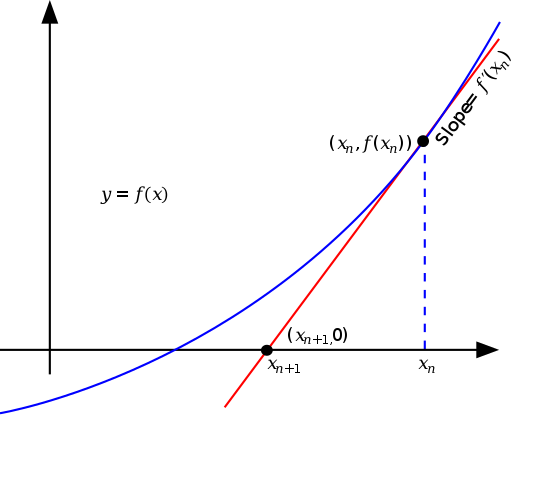
\includegraphics[width=0.5\textwidth]{mn1.png}}
	\caption{Demostración del método de Newton-Raphson}
	\label{mn1}
\end{figure}

El método de Newton-Raphson, genera una sucesión de valores en el eje horizontal,
la cual se espera que converja al $x^*$ tal que $f(x^*)\thickapprox 0$.

\begin{equation}
	x_1,x_2,x_3,\dots x_N, x_{N+1},x_{N+2} \dots x^*
\end{equation}

Sea $x_1$ el valor inicial (Muy cernano a $x^*$), como $f(x)$
es una función de clase $C^1\implies \exists P \in $ gráfica de $f(x) \mid (x_1, f(x_1))$
y dado ese punto, $\exists f^{\prime}(x)=$. Por lo tanto la pendiente de la recta tangente
a $f$ en el punto $x_1, f(x_1))$, luego la ecuación de la recta tangente será

\begin{equation}
	y-y_1=m\left(x-x_1\right)
\end{equation}

La recta tangente intersecta en el eje horizontal

\begin{align*}
	 & y=0                                                             \\
	 & \implies 0-f(x_0)=f^{\prime}(x_0)(x-x_0) \text{ y se despeja x} \\
	 & \text{Siempre que } f^{\prime}(x_0)\neq 0 \text{ entonces }     \\
	 & -\frac{f(x_1)}{f^{\prime}(x_1)}=x-x_1                           \\
	 & \therefore x_2=x_1-\frac{f(x_1)}{f^{\prime}(x_1)}
\end{align*}

El proceso comenzará nuevamente considernado a $x_2$ como la aproximación inicial, es decir:
se tiene un punto $p$ sobre la curva a saber $x_2$

La cual intersecta al eje horizontal cuando $y=0$

\begin{equation}
	\therefore x_3=x_2-\frac{f(x_2)}{f^{\prime}(x_3)}
\end{equation}

en forma general, la fórmula de Newton-Raphson:

\begin{equation}
	x_n=x_{n-1}-\frac{f(x_{n-1})}{f^{\prime}(x_{n-1})}
\end{equation}

\begin{example}
	Aplique el método de Newton-Raphson para encontrar las soluciones ``exactas'' dentro de $10^{-5}$ para la ecuación

	\begin{equation*}
		x^4-2x^3+4x+4=0
	\end{equation*}
\end{example}

\textit{ Sol. }

Precisión o tolerancia:

Todas las raíces de una ecuación polinomial cumple con:

\begin{enumerate}
	\item Regla de los signos de Descartes, de más a menos hay una variación, de menos a más hay otra variación, pero de más a más, hay una permanencia

	      Conclusión, la ecuación tiene a lo más, dos raíces reales positivas.
	\item El teorem da acotación de raíces:
	      \begin{theorem}[Acotación de raíces]
		      \begin{equation}
			      R=1+\max \left\{ \left\lvert \frac{a_{n-1}}{a_n} \right\rvert,\left\lvert \frac{a_{n-1}}{a_n} \right\rvert, \dots , \left\lvert \frac{a_{0}}{a_n} \right\rvert  \right\}
		      \end{equation}
	      \end{theorem}
	      donde $p_n(x)= a_{n}x^n+a_{n-1}x^{n-1}+a_{n-2}x^{n-2}+\dots+a_{2}x^2+a_{1}x+a_0$
	      Para este caso:
	      \begin{align*}
		       & a_4=1,a_3=-2,a_2=0,a_1=4,a_0=4                                                                                                                                             \\
		       & R=1+\max \left\{ \left\lvert \frac{-2}{1}\right\rvert,\left\lvert \frac{0}{1}\right\rvert,\left\lvert \frac{4}{1}\right\rvert,\left\lvert \frac{4}{1}\right\rvert \right\} \\
		       & R=2+\max \left\{2,0,4,4\right\}=1+4=5
	      \end{align*}
	      Conclusión: Todas las raíces se encuentran en el intervalo [-5,5]

	      Se supondrá que $f(x)=x^4-2x^3++4x+4$ y resolver la ecuación, implicará gráficamente
	      encontrar las intersecciones de la gráfica de $f$ con el eje horizontal.

	      Se proponen evaluaciones de $f(x)$ en el intervalo [-5,5] con los multiplos
	      divisores del término independiente son: -4,-2,-2,1,2,4

	      Conclusión: Al no haber cambio de signo en las \textbf{evaluaciones} realizadas en el intervalo donde se localizan todas las raíces reales positivas y negativas de $f(x)$, se
	      concluye que $f(x)$ no tiene raíces, es decir no tiene solución en los reales.
\end{enumerate}

\begin{example}
	Encuentre las soluciones de la ecuación:
	\begin{equation*}
		x^4+2x^3-x-3=0
	\end{equation*}
	Empleando el método de Newton-Raphson, usando aritmética de 8 decimales y una precisión de $10^{-5}$
\end{example}

\textit{ Sol. }

\begin{enumerate}
	\item Regla de los signos de Descartes: +,+,-,-

	      Sólo puede tener a lo más una raíz real positiva.

	\item Teorema de acotación de raíces:

	      \begin{align*}
		       & R=1+\max \left\{\left\lvert \frac{2}{1}\right\rvert,\left\lvert \frac{0}{1}\right\rvert, \left\lvert \frac{-1}{1}\right\rvert,\left\lvert \frac{-3}{1}\right\rvert \right\} \\
		       & R=1+\max \left\{2,0,1,3\right\}=1+3=4
	      \end{align*}

	      Todas las raíces se encuentran en el intervalo [-4,4]

	      Se supondrá que $f(x)=x^4+2x^2-x-3$ y se evaluarán los divisores de 3 en el intervalo [-4,4]
	      \begin{enumerate}
		      \item f(-3)=99
		      \item f(-1)= 1
		      \item f(1)=-1
		      \item f(3)=93
	      \end{enumerate}
	      Con este procedimiento se han encontrado dos cambios de signo en la función $f(x)$,
	      y con ello dos intervalos+ donde se localizan las raíces de la ecuación (o bien con el eje horizontal)
	      Una intersección pcurre en el intervalo (-1,1) y la otra intersección ocurre en el intervalo (1,3)

	      En cada intervalo se tiene que dar una aproximación inicial ``arbitraria''.
	      para el primer intervalo sea $x_1=-0.7$ por elección,
	      Para el segundo intervalo sea $x_1=2.1$ por elección.

	\item a
	\item a
\end{enumerate}

%%%%%%%%%%muchas operaciones después, revisar los apuntes classroom

Para $n=2$

\begin{align*}
	x_2 & =-0.7-2.0879737 \\
	x_2 & =-0.90879737
\end{align*}

Para $n=3$

\begin{align*}
	x_3 & =-0.90879737-\frac{0.24275441}{-7.63753849} \\
	x_3 & =-0.90879737+0.03178438                     \\
	x_3 & =-0.90879737
\end{align*}

para $n=4$

\begin{align*}
	x_4 & =-0.87701299-\frac{0.00691103}{-7.20627639} \\
	x_4 & =-0.87605396
\end{align*}

para $n=5$

\begin{align*}
	x_5 & =-0.87605396-\frac{0.00000607}{-7.19359827} \\
	x_5 & =-0.87605396+0.00000084                     \\
	x_5 & =-0.87605312
\end{align*}

Para $x_6$

\begin{align*}
	x_6 & =-0.87605312-\frac{0.00000003}{-7.19358717} \\
	x_6 & =-0.87605312-0.00000000                     \\
	x_6 & =-0.87605312
\end{align*}


\begin{table}[h!]
	\centering
	\begin{tabular}{|c|c|c|c|}
		\hline
		Iteración & $x_n$       & $\left\lvert f(x_n)\right\rvert $ & 0.00001 \\ \hline
		1         & -70000000   & 1.07990000                        & NO      \\ \hline
		2         & -0.90879737 & 0.24275441                        & NO      \\ \hline
		3         & -0.87701299 & 0.00691103                        & NO      \\ \hline
		4         & -0.87605396 & 0.00000607                        & SI      \\ \hline
	\end{tabular}
	\caption{Tabla de resultados}
	\label{tabfmc18}
\end{table}


%%%%%%%%%%%%FINAL PENDIENTE, REVISAR

\begin{problem}[Use el método de N-R para encontrar una aproximación de $10^{-5}$ a la solución de la ecuación]
\begin{equation*}
	-e^{-x}+\sin(x)=0
\end{equation*}
Usando aritmética de siete decimales
\end{problem}

\textit{ Sol. }

La ecuación tres al no ser una ecuación polinomial, no es posibles4aplicar el teorema de acotación de raíces ni la regla de
los signos de Descartes.

\begin{enumerate}
	\item Se asocia una función a la ecuación, para éste caso: $g(x)=\sin(x)-e^{-x}$
	\item Ahora se intentará biscar un cambio de signo en $g(x)$ con diferentes valores de $x$
	      \begin{align*}
		      g(0)=\sin(0)-e^{-0}=-1         \\
		      g(1)=\sin(1)-e^{-1}=0.4735915
		      g(2)=\sin(2)-e^{-2}=0.7739621  \\
		      g(3)=\sin(3)-e^{-3}=0.0913329  \\
		      g(4)=\sin(4)-e^{-4}=-0.7751181 \\
	      \end{align*}

	      Con las evaluaciones realizadas se observan dos cambios de signo en la función;
	      por lo tanto ls intervalos donde se localizan algunas soluciones de la ecuación son:

	      (0,1) Y (3,4)

	\item Para aplicar la fórmula de N-R, es necesario calcular la $I^2$ derivada de $g(x)$

	      \begin{equation*}
		      g^{\prime}(x)=\cos(x)+e^{x}
	      \end{equation*}

	      La fórmula para este caso es:

	      \begin{equation*}
		      X_n=x_{n-1}-\frac{\sin(x_{n-1}-e)}{\cos(x_{n-1}+e^{-x_{n-1}})}
	      \end{equation*}

	\item Hacemos dos aproximaciones con intervalo de 0 a 1 y de 3 a  4

	      \begin{table}[h!]
		      \centering
		      \begin{tabular}{@{}llll@{}}
			      \toprule
			      $n$        & \textbf{$x_n$} & \textbf{$\left\lvert f(x:n)\right\rvert $} & \textbf{$\left\lvert f(x:n)\right\rvert<0.00001$} \\ \midrule
			      \textbf{1} & 0.7000000      & 0.1476324                                  & NO                                                \\
			      \textbf{2} & 0.5829640      & 0.0077405                                  & NO                                                \\
			      \textbf{3} & 0.5885204      & 0.0000171                                  & NO                                                \\
			      \textbf{4} & 0.5885327      & 0.00000000                                 & SI                                                \\ \bottomrule
		      \end{tabular}
		      \caption{Una aproximación $10^{-5}$ de una solución es igual a $x_4=0.5885327$}
		      \label{tabfmc19}
	      \end{table}


	      \begin{table}[h!]
		      \centering
		      \begin{tabular}{@{}llll@{}}
			      \toprule
			      $n$        & \textbf{$x_n$} & \textbf{$\left\lvert f(x:n)\right\rvert $} & \textbf{$\left\lvert f(x:n)\right\rvert<0.00001$} \\ \midrule
			      \textbf{1} & 3.5000000      & 0.3809806                                  & NO                                                \\
			      \textbf{2} & 3.0796119      & 0.0159640                                  & NO                                                \\
			      \textbf{3} & 3.0963790      & 0.0000144                                  & NO                                                \\
			      \textbf{4} & 3.0963639      & 0.00000000                                 & SI                                                \\ \bottomrule
		      \end{tabular}
		      \caption{Una aproximación $10^{-5}$ de una solución es igual a $x_4=3.0963639$}
		      \label{tabfmc20}
	      \end{table}
\end{enumerate}

\section{Derivación implícita}

Considérese la ecuación $F(x,y)=0$ la cual determina a $y$ como la función implícita de $x$
y que será diferenciable, tal que al derivar de ambos lados se obtiene una ecuación de primer grado
con respecto a  $y^{\prime}$ (derivada implícita)

Algunas expresiones implícitas son:

\begin{align*}
	 & \underbrace{x3+\ln(y)-x^2e^y}_{f(x,y)=f(x,y(x))}=0  \\
	 & \underbrace{x^3+y^3-3xy=0}_{f(x,y)=f(x,y(x))} =0    \\
	 & \underbrace{x\sin(y)-y\sin(x)}_{f(x,y)=f(x,y(x))}=0
\end{align*}

\begin{remark}
	Al ser $y=y(x)$se deriva $y^{\prime}=\frac{dy}{dx}$
\end{remark}

\begin{example}
	Calcular $y^{\prime}$ para las expresión:

	\begin{align*}
		 & x^3+\ln(y)-x^2e^y=0\text{ Derivando respecto a y: }                                                      \\
		 & 3x^2+\frac{y^{\prime}}{y}-\left(2xe^y+x^2e^y\cdot y^{\prime}\right)=0 \text{ Agrupando y factorizando: } \\
		 & y^{\prime}\left(\frac{1}{y-X^2e^y} \right)=-3x^2+2xe^y                                                   \\
		 & y^{\prime}=\frac{-3x^2+2xe^y}{\frac{1}{y}+x^2e^y}
	\end{align*}
\end{example}

\begin{example}
	Calcular $y^{\prime}$ para las expresión:

	\begin{align*}
		 & x^3+y^3-3xy=0 \text{ Derivando respecto a y: }                                             \\
		 & 3x^2+3y^2\cdot y^{\prime}-3\left(y+xy^{\prime}\right)=0 \text{ Agrupando y factorizando: } \\
		 & y^{\prime}\left(3y^2-3x\right)=-3x^2+3y \text{ Despejando }y^{\prime}                      \\
		 & y^{\prime}=\frac{y-x^2}{y^2-x}
	\end{align*}
\end{example}

\subsection{Aplicaciones diversas de la derivdada}

\begin{example}
	Cacule la ecuación de la recta tangente que pasa por el punto (4,14)
	y es tangente a la curva $y(x)=x^2+4x+7$
\end{example}

\textit{ Sol. }

Se deriva la ecuación $y(x)=x^2+4x+7$ y se obtiene

\begin{equation*}
	y^{\prime}(x)=2x+4
\end{equation*}

Se sabe que $y^{\prime}(x)$ es la pendiente de la recta tangente en cuaqluier punto de $y(x)$
y por otro lado la pendiente de la recta tangente en el punto $(x_0,y_0)$ que pasa por el punto
$(4,14)$ es:

\begin{equation*}
	m=\frac{14-y_0}{4-x_0}=2x_0+4\implies \frac{14-(x_0+4x_0+7)}{4-x_0}=2x_0+4
\end{equation*}

simplificando

\begin{equation*}
	x_0^2-8x_0-9=0
\end{equation*}

Se tiene una ecuación cuadrática para $x_0$ la ucal hay que resolver:
$x_0^1=-1$ y $x_0^2=9$ Son la coordenada x de los puntos de tangencia.

Finalmente los pintos de tangencia serán:

\begin{align*}
	y(-1)=(-1)^2+4(-1)+7=4\text{ y con el otro punto:} \\
	y(9)=(9)^2+4(9)+7=81+36+7=123
\end{align*}

Se tiene el punto (-1,4) y (0,124)

Ahora se determinan las ecuaciones de la recta tangente para el punto (-1,4)

\begin{align*}
	y^{\prime}(-1)=2(-1)+4=2=M
\end{align*}

La recta tangente es $y-4=2(x-(-1))$ eso es $y=2x+6$

Para el punto (9,124) la pendiente será $y^{\prime}(9)=2(9)+4=22$ eso es $y=22x-74$

Ahora se determinan los valores críticos de $A$

\begin{align*}
	 & A^{\prime}=\frac{12x(x-2)-6x^2}{[2(x-2)]^2 }\implies A^{\prime}=\frac{6x^2-24x}{4(x-2)^2}=0 \\
	 & \implies x=0\land x=4
\end{align*}

Ahora para clasificar los puntos críticos

\begin{align*}
	 & A^{\prime\prime}=\frac{(6x-12)(2)(x-2)^2-(3x^2-12x)(4)(x-2)}{[2(x-2)^2]^2}\implies \\
	 & A^{\prime\prime}=\frac{(12x-24)(x-2)-(12x^2-18x)}{4(x-2)^3}                        \\
	 & A^{\prime\prime}= \frac{12}{(x-2)^3}
\end{align*}

Evaluando los valores críticos $x=0$ y $x=4$ en $A^{\prime\prime}$ para clasificarlos
$A^{\prime\prime}(0)=\frac{12}{8}<0$ por lo tanto $x=0$ habrá un máximo y en $x=0$ no hay triángulo, por lo tanto queda descartado.

Evaluando en 4, tenemos que $\frac{12}{8}>0$ y con la realción de las pendientes se obtiene $y=6$


Una intersección de la recta que pasa por el punto (2,3) con el eje horizontal es en $x=4$, en tanto que la intersección con el
eje vertical es $y=\frac{6}{x-2}-3\implies y=6$ finalmente el área del triángulo será $A=12u^2$

\begin{example}
	Calcule
\end{example}

\section{Aplicación a problemas de optimización}

\begin{example}
	¿Cuál es el área máxima de un rectangulo cuya base está en el eje $x$ y con dos vértices superiores en la gráfica de la ecuación $y=4-x^2$?
\end{example}

\textit{ Sol. }

La idea gráfica: al ser simétrica la base la partimos en dos.

El objetivo es maximizar el área, sujeto a una restricción.

Sean $x_0=$ la mitas de la base del rectángulo y $y_0=$ la altura del rectángulo

El modelo matemático.

$\max A(x_0,y_0)=x_0y_0$ y $y_0=4-x_0^2$ tenemos la desigualdad $x_,y_0>0$

Como la función de área depende de dos variables y sólo se puede trabajar con una variable independiente
entonces:

\begin{align*}
	A=(x_0,y_0)=A(x_0,4-x^2_0)=x_0(4-x^2_0)=A(x_0)                                                 \\
	\implies A(x_0)=4x_0-x^3, x_0 \in (0,2)                                                        \\
	A^{\prime}(x_0)=4-3x_0^2=0\implies x_0^2=\frac{4}{3}\implies                                   \\
	x_0=\pm \frac{2}{\sqrt{3}} \text{ ërp eñ valor }\frac{-2\sqrt{3}}{3} \text{ queda descartado } \\
	\frac{-2\sqrt{3}}{3}\notin (0,2) \text{ Por lo tanto } x_0=\frac{2\sqrt{3}}{3}                 \\
	\text{Ahora se verifica que }x_0=\frac{2\sqrt{3}}{3}=-6\left(\frac{2\sqrt{3}}{3}<0\right)
\end{align*}

En $x_0=\frac{2\sqrt{3}}{3}$ hay un máximo locas, las dimensiones del rectángulo de área máximo son:

\begin{align*}
	 & x=\frac{4\sqrt{3}}{3} &  & y=4-\left(\frac{4\sqrt{3}}{3}\right)^2 \\
	 & x=\frac{4\sqrt{3}}{3} &  & y=\frac{24}{9}
\end{align*}

Y el área máxima será:

\begin{equation*}
	A=\left(\frac{4\sqrt{3}}{3}\right)\left(\frac{24}{9}\right)=\frac{32\sqrt{3}}{9}u^2
\end{equation*}

\begin{example}
	Se requiere fabricar un contenedor cerrado de acero de volumen específico y en forma de cilíndro círcular recto.
	Hallar la razón de la altura al radio de la base, sí se desea emplear la menor cantidad de material posible para su fabricación.
\end{example}

\textit{ Sol. }

Se divide el dibujo en un rectangulo $A_R$ y un círculo $A_C$:

\begin{align*}
	 & A_R(r,h)=2\pi rh &  & A_C(r,h)=\pi r^2
\end{align*}

El área superficial del cilindro es:

\begin{equation*}
	A_s(r,h)=2\pi rh+2\pi r^2
\end{equation*}

El modelo matemático es:

\begin{align*}
	V(r,h)=\pi r^2h=K \mid r,h\geq 0
\end{align*}

Como el volumen es constante, entonces $h=\frac{k}{\pi r^2}$ y se sustituye $h$ en la función objetivo, se obtiene:

\begin{equation*}
	A_s(r,h)=A_s\left(r,\frac{k}{\pi r^2}\right)=2\pi r\left(\frac{k}{\pi r^2}\right)+2\pi r^2=A_s(r)
\end{equation*}

simplificando

\begin{equation*}
	A_S(r)=\frac{2k}{r}+2\pi r^2
\end{equation*}

Derivando e igualando a cero se obtiene

\begin{equation*}
	r=\sqrt[3]{\frac{k}{2\pi}}
\end{equation*}

Ahora se calcula la segunda derivada para calsificar el valor crítico encontrado:

\begin{equation*}
	A_s^{\prime\prime}(r)=4\pi+\frac{4k}{r^3}
\end{equation*}

Evaluando el valor crítico en la segunda derivada

\begin{equation*}
	A_s^{\prime\prime}\left(\sqrt[3]{\frac{k}{2\pi}}\right)=12\pi>0\therefore \text{ Es un mínimo}
\end{equation*}

Se sabe que $r=\sqrt[3]{\frac{k}{2\pi}};h=\frac{k}{\pi\left(\frac{k}{2\pi} \right)^2}$

Por lo tanto $\frac{h}{r}$ será:

\begin{align*}
	 & \frac{h}{r}=\frac{\frac{k}{\pi\left(\sqrt[3]{\frac{k}{2\pi}}\right)^2}}{\frac{\frac{k}{2\pi}}{1}} \\
	 & \frac{h}{r}=\frac{k}{\pi\left(\sqrt[3]{\frac{k}{2\pi}}\right)^3}                                  \\
	 & \cdots                                                                                            \\
	 & h=2r
\end{align*}

\subsection{Multiplicadores de lagrange}

\begin{example}
	Se fabricará una lata cilíndrica con tapa que contenga un litro de aceite. Calcule las dimensiones que minimicen el costo del metal empleado en la fabricación de la lata.
\end{example}

\textit{ Sol. }

Modelo matemático
\begin{align*}
	\min A(r,h)=2\pi r^2+2\pi rh \text{ Función objetiva} \\
	V(r,h)=\pi r^2h=1 \text{ Restricción}                 \\
	r>0,h>0 \text{ Condiciones de no negatividad}
\end{align*}
Se formará una ecuación auxiliar:
\begin{align*}
	\mathfrak{L} (r,h)=2\pi r^2+2\pi rh-\lambda \left(\pi r^2h-1\right)
\end{align*}

Ahora se resuelve un sistema de ecuaciones

\begin{equation*}
	\frac{\partial \mathfrak{L} }{\partial r}=4\pi r+2\pi h+2\pi \lambda hr=0\\
	\frac{\partial \mathfrak{L} }{\partial r}=2\pi r+\lambda \pi r^2=0\\
	\frac{\partial \mathfrak{L} }{\partial r}=\pi r^2h-1=0
\end{equation*}

De la segunda ecuación aquí planteada, sabemos que $2+\lambda r=0$

Ahora se sustituye esta nueva ecuación en la primera:

\begin{equation*}
	2r+h-2h=0\implies 2r-h=0\implies h=2r
\end{equation*}

Finalmente se sustituye la nueva ecuación en la tercera:

\begin{equation*}
	\pi r^2(2r)-1=0\implies 2\pi r^3-1=0\implies r=\sqrt[3]{\frac{1}{2\pi}}
\end{equation*}

Las dimensiones de la lata con volumen dijo de un litro es:

\begin{align*}
	 & r=\frac{1}{\sqrt[3]{2\pi}} &  & h=\frac{2}{\sqrt[3]{2\pi}}
\end{align*}
\newpage
\section{El teorema de Taylor}

\begin{theorem}[Teorema de Taylor]
	Sea $f$ una función tal que $f$ y sus primeras $n$-derivadas son continuas en el intervalo $[a,b]$.
	Además considere que $f^{n+1}(x)$ existe para toda $x\in (a,b)$. Entonces
	existe un número $\xi$ en el intervalo $(a,b)$ tal que:

	\begin{equation}
		f(b)=f(a)+\frac{f^{\prime}(a)}{1!}\left(b-a\right)+\frac{f^{\prime\prime}(a)}{2!}\left(b-a\right)^2+\cdots+\frac{f^{n}(a)}{n!}+\frac{f^{n+1}(\xi)}{\left(n+1\right)!}\left(b-a\right)^{n+1}
	\end{equation}

	Si en la expresión anterior se reemplaza a $b$ por $x$, entonces se obtiene el polinómio de Taylor de grado $n$, es decir:

	\begin{equation}
		f(x)=\underbrace{P_n(x)}_{\text{Polinomio de Taylor}}+\underbrace{R_{n+1}(\xi)}_{\text{Residuo de lagrange}}
	\end{equation}

	\begin{equation}
		f(x)=f(a)+\frac{f^{\prime}(a)}{1!}\left(x-a\right)+\frac{f^{\prime\prime}(a)}{2!}\left(x-a\right)^2+\cdots+\frac{f^n(a)}{n!}\left(x-a\right)^n+\underbrace{\frac{f^{n+1}\xi}{\left(n+1\right)!}\left(x-a\right)^{n+1}}_{\text{Residuo de lagrange}}
	\end{equation}
\end{theorem}

\begin{example}
	Calcule le polinómio de Taylor de grado $n$ para la función $f(x)=e^x$
\end{example}

\textit{ Sol. }

Analizando sus derivadas, obtenemos:

\begin{align*}
	 & f^{\prime}(x)=e^x,f^{\prime\prime}(x)=e^x,\cdots,f^n(x)=e^x, f^{n+1}(x)=e^x                                                                                     \\
	 & e^x=P_n(x)+R_{n+1}(x)                                                                                                                                           \\
	 & e^x=e^a+e^a\left(x-a\right)+\frac{1}{2}e^a\left(x-a\right)^2+\cdots+\frac{1}{n!}e^a\left(x-a\right)^n+\frac{1}{\left(x+1\right)!}e^{\xi} \left(x-a\right)^{n+1}
\end{align*}

Sí $a=0\implies $ se obtiene un polinomio en particula, llamado polinomio de Mc. Lavrin para $f(x)=e^x$ será:

\begin{equation*}
	e^x=e^0+e^0\left(x-0\right)+\frac{1}{2}e^0\left(x-0\right)^2+\cdots+\frac{1}{n!}e^0\left(x-0\right)^n+\frac{1}{\left(n+1\right)!}e^{\xi} \left(x-0\right)^{n+1}
\end{equation*}

simplificando:

\begin{equation*}
	e^x=\underbrace{1+x+\frac{1}{2}x^2+\cdots+\frac{1}{n!}x^n+\frac{1}{\left(n+1\right)!}e^{\xi} x^{n+1}}_{\text{Serie de Mc. Lavrin de $e^x$ alrededor de 0}}
\end{equation*}

\section{polinomio de Mc. Laurin}

Use el polinomio de Mc. Lavrin (de grado adecuado) para aproximar el valor de $e^{0.7}$

\begin{align*}
	 & e^0.7\approx 1+0.7+R_2(0.7)                                         \\
	 & e^0.7\approx 1+0.7+\frac{1}{(1+1)!}e^{\xi} (0.7)^2; \xi \in (0,0.7) \\
	 & e^0.7=2.01375271                                                    \\
	 & \text{Con el polinomio de Mc Laurin de grado 1: }                   \\
	 & 1+0.7+\frac{1}{2!}e^{0.5}(0.7)^2=1.7+\frac{1}{2}(1.64872127)(0.49)  \\
	 & =1.7+\underbrace{0.40393671}_{\text{Residuo de Lagrange}}           \\
	 & =2.10393671
\end{align*}

El mismo ejercicio pero con un polinomio de Mc. Lavrin de grado dos:

\begin{equation*}
	e^x\approx 1+x+\frac{1}{2}x^2+R_3(x); R_{3}(x)=\frac{1}{3!}e^{\xi}x^3;\xi\in(0,x)
\end{equation*}

si $x=0.7\implies e^0.7$

\begin{equation*}
	\approx1+0.7+\frac{1}{2}(0.7)^2+R_3(0.7); \text{ Donde } R_3(0.7)=\frac{1}{6}e^{\xi} (0.7)^3
\end{equation*}
como $\xi \in (0,0.7)$, entonces:

\begin{equation*}
	e^0.7\approx1.7+0.245+0.05716667E^{\xi}; \xi\in (0,0.7)
\end{equation*}

Si tomamos un valor albitrrio: $\xi =0.5$

\begin{align*}
	e^0.7 \approx 1.945+0.05716667e^0.5 \\
	e^0.7 \approx 1.945+0.09425180      \\
	e^0.7 \approx 2.03925190
\end{align*}

\begin{example}
	Determine un polinomio de Mc. Lavrin de grado cinco para $g(x)=\sin(x)$
\end{example}

\textit{ Sol. }

Se calculan todas sus derivadas:

\begin{align*}
	 & g(x)=\sin(x)                       &  & g^{\prime}(x)=\cos(x) &  & g^{\prime\prime}(x)=-\sin(x) \\
	 & g^{\prime\prime\prime}(x)=-\cos(x) &  & g^4(x)=\sin(x)        &  & g^5(x)=\cos(x)               \\
	 & g^6(x)=-\sin(x)
\end{align*}

Evaluando en cero:

\begin{align*}
	\sin(x)=0.1\cdot x+0-\frac{1}{6}x^3+0+\frac{1}{120}x^5+R_6(x) \\
	\text{Donde } R_6(x)=-\frac{1}{7!}\sin(\xi)x^6                \\
	\sin(x)\approx x-\frac{1}{6}x^3+\frac{1}{120}x^5-\frac{1}{6!}(\xi); \xi \in (0,x)
\end{align*}

En general el desarrollo en seria de Mc. Lavrin para $\sin(x)$ es:

\begin{equation*}
	\sin(x)\approx x-\frac{1}{3!}x^3+\frac{1}{5!}x^5-\frac{1}{7!}x^7+\frac{1}{9!}x^9+\cdots+R_{n+1}(x)
\end{equation*}

\subsubsection{Desplazamiento de la serie}

Si se desea calcular $\sin(47^{\circ})=\sin(45^{\circ}+2^{\circ})$, Así que denotamos a $x=45^{\circ}+2^{\circ} \implies x-45^{\circ}=2^{\circ}$
y por lo tanto $\implies x=\frac{47\pi}{180}$

El polinomio de Taylor en su expresión general es:
\begin{align*}
	 & f(x)\approx f(a)+\frac{1}{1!}f^{\prime}(a)(x-a)+\frac{1}{2!}f^{\prime\prime}(a)(x-a)^2+\cdots+\frac{1}{n!}f^n(a)(x-a)^n+R_{n+1}(x) \\
	 & \text{Donde }R_{n+1}(x)=\frac{1}{(n+1)!f^{n+1}(\xi)(x-a)^{n+1}\text{ Con } \xi\in (a,x)}
\end{align*}

Para éste ejemplo, la aproximación será de $a=45^{\circ}$ o bien $\frac{\pi}{4}$rad, entonces:

\begin{align*}
	 & \sin(x)\approx \sin\left(\frac{\pi}{4}\right)+\frac{1}{1!}\cos\left(\frac{\pi}{4}\right)\left(x-\frac{\pi}{4}\right)+\frac{1}{2!}\left(-\sin \left(\frac{\pi}{4}\right)\right)\left(x-\frac{\pi}{4}\right)^2+\dots                                       \\
	 & \dots+\frac{1}{3!}\left(-\cos\left(\frac{\pi}{4}\right) \right)\left(x-\frac{\pi}{4}\right)^3+\frac{1}{4!}\sin \left(\frac{\pi}{4}\right)\left(x-\frac{\pi}{4}\right)^4+\frac{1}{5!}\cos \left(\frac{\pi}{4}\right)\left(x-\frac{\pi}{4}\right)^5+R_6(x)
\end{align*}

Donde $R_6(x)=\frac{1}{6!}\left(-\sin(\xi)\right)\left(x-\frac{\pi}{4}\right)^6$ con $\xi \in \left(\frac{\pi}{4},x\right)$


La expresión anterior es un polinomio de Taylor de grado 5. Desplazando $\frac{\pi}{4}$ unidades del orígen. Ahpra se emplearáéste polinomio para calcular $\sin\left(\frac{47\pi}{180}\right)$

\begin{align*}
	 & \sin\left(\frac{47\pi}{180}\right) \approx \frac{\sqrt{2}}{2}+\frac{\sqrt{2}}{2}\left(x-\frac{\pi}{4}\right)-\frac{\sqrt{2}}{4}\left(x-\frac{\pi}{4}\right)^2-\frac{\sqrt{2}}{12}\left(x-\frac{\pi}{4}\right)^3+\frac{\sqrt{2}}{48}\left(x-\frac{\pi}{4}\right)^4+\dots \\
	 & \dots+\frac{\sqrt{2}}{240}\left(x-\frac{\pi}{4}\right)^5+R_6(x);\xi \in \left(\frac{\pi}{4},x\right)                                                                                                                                                                    \\
	 & \sin \left(\frac{47\pi}{180}\right)=\frac{\sqrt{2}}{2}\left(1+\left(\frac{47}{180}\pi-\frac{\pi}{4}\right)-\frac{1}{2}\left(\frac{47}{180}\pi-\frac{\pi}{4}\right)^2-\frac{1}{6}\left(\frac{47}{180}\pi-\frac{\pi}{4}\right)^3\right)\dots                              \\
	 & \dots+\frac{\sqrt{2}}{2}\left(\frac{1}{24}\left(\frac{47}{180}\pi-\frac{\pi}{4}\right)^4+\frac{1}{120}\left(\frac{47}{180}\pi-\frac{\pi}{4}\right)^5\right)+R_6(x)\text{ con } \xi \in \left(\frac{\pi}{4},\frac{47\pi}{180}\right)                                     \\
	 & \sin \left(\frac{47\pi}{180}\right)=\frac{\sqrt{2}}{2}\left[1+\frac{\pi}{90}-\frac{1}{2}\left(\frac{\pi}{90}\right)^2-\frac{1}{6}\left(\frac{\pi}{90}\right)^3+\frac{1}{24}\left(\frac{\pi}{90}\right)^4 +\frac{1}{120}\left(\frac{\pi}{90}\right)^5\right]+\dots       \\
	 & \dots+R_6(x), \text{ con } \xi \in \left(\frac{\pi}{4},\frac{47}{180}\pi\right)                                                                                                                                                                                         \\
	 & \sin \left(\frac{47}{180}\pi\right)\approx 0.73135370+R_6(x) \text{ con } \xi\in \left(\frac{\pi}{4},\frac{47}{180}\pi\right)
\end{align*}

Con calculadora, directamente:

\begin{equation*}
	\sin \left(\frac{47}{180}\pi\right)=0.73135370
\end{equation*}

\section{Regla de L' Hôptal}

\begin{theorem}[L' Hôpital]
	\begin{itemize}
		\item Sean $f$ y $g$ funciones diferenciables en el intervalo abierto $I$, excepto posiblemente en el valor $``a^{\prime\prime}\in I$, y suponga que $\forall x \neq 0$. Si $\lim_{x\to a}f(x)=\infty$ o $-\infty$ y
		      \begin{equation}
			      \lim_{x\to a}\frac{f^{\prime}(x)}{g^{\prime}(x)}=L\implies \lim_{x\to a}\frac{f(x)}{g(x)}=L
		      \end{equation}

		      Es el apartado del teorema para formas indeterminadas del tipo $\frac{\infty}{\infty}$

		\item a Si \begin{align*}
			       & \lim_{x\to a} f(x)=0                                &  & \lim_{x\to a}g(x)=0                        \\
			       & \lim_{x\to a} \frac{f^{\prime}(x)}{g^{\prime}(x)}=L &  & \implies \lim_{x\to a} \frac{f(x)}{g(x)}=L
		      \end{align*}

		      Es el apartado del teorema para formas indeterminadas del tipo $\frac{0}{0}$

	\end{itemize}
\end{theorem}

\begin{example}
	Calcule los siguientes límites:
	\begin{enumerate}
		\item $\lim_{x\to 0}\frac{\sin(x)}{x}=$

		      \textit{ Sol. }
		      \begin{equation*}
			      \lim_{x\to 0}\frac{\sin(x)}{x}=\frac{\sin(x)}{x}=\frac{\sin(0)}{0}=\frac{0}{0}
		      \end{equation*}

		      Aplicando la regla de L Hôpital para calcular el límite:

		      \begin{align*}
			       & \lim_{x\to 0}\frac{\sin(x)}{x}=\lim_{x\to 0}\frac{\cos(x)}{1}=\lim_{x\to 0}\frac{\sin(0)}{1}=\frac{1}{1}=1 \\
			       & \therefore \lim_{x\to 0}\frac{\sin(x)}{x}=1
		      \end{align*}

		\item $\lim_{x\to 1}\frac{\ln(x)}{x-1}=$

		      \textit{ Sol. }

		      \begin{align*}
			       & \lim_{x\to 1}\frac{\ln(x)}{x-1}=\frac{0}{0}                          \\
			       & \lim_{x\to 1}\frac{\ln(x)}{x-1}=\lim_{x\to 1}\frac{\frac{1}{x}}{1}=1 \\
			       & \lim_{x\to 1}\frac{\ln(x)}{x-1}=1
		      \end{align*}
	\end{enumerate}

\end{example}

\section{Razón de cambio (Tasa de variación)}

\begin{definition}[Razón de cambio]
	Si $y=f(x)$ entonces la razón de cambio instantánea de $y$ por unidad de variación de $x$ en el valor de $x_1$ es $y'(x)=f^{\prime}(x)$ siempre y cuando la derivada exista.
\end{definition}

\begin{example}
	Sea $V(x)$ centímetros cúbicos el volumen de un cubo cuyas arístas miden $``x''$ centímetros, medidas con cuatro dígitos significativos. Obtenga la tasa de variación de $V(x)$ con respecto a $``x''$ conforme $x$ varía de:
	\begin{enumerate}
		\item 3.00 a 3.200
		\item 3.000 a 3.100
		\item 3.00 a 3.010
		\item ¿Cuál es la razón de cambio instantánea de $V(x)$ con respecto a $x$ cuadno $x=3.000$?
	\end{enumerate}
\end{example}

\textit{ Sol. }

La razón de cambio promedio de $V(x)$ con respecto a $x$ cuando varía de $x$ a $x_1=x+\delta x$

\begin{equation*}
	\frac{\delta V}{\delta X}=\frac{V\left(x_1+\delta x\right)-V_(x_1)}{\delta x}
\end{equation*}

Para éste caso concreto, $x_1=3.000$ pero $\delta x$ es distinto en cáda caso.

\begin{enumerate}
	\item $\delta x= 3.200-3.000=0.200$
	\item $\delta x= 3.100-3.000=0.100$
	\item $\delta x= 3.010-3.000=0.010$
\end{enumerate}

Por lo tanto:

\begin{enumerate}
	\item $\frac{\delta V}{\delta x}=\frac{V(3.200)-V(3.000)}{0.200}=\frac{(3.200)^3-(3.000)^3}{0.200}=28.84$
	\item $\frac{\delta V}{\delta x}=\frac{V(3.100)-V(3.000)}{0.100}=\frac{(3.100)^3-(3.000)^3}{0.100}=27.91$
	\item $\frac{\delta V}{\delta x}=\frac{V(3.010)-V(3.000)}{0.010}=\frac{(3.010)^3-(3.000)^3}{0.010}=27.09$
\end{enumerate}

Sustituyendo $V(x)=x^3 \implies V^{\prime}(x)=3x^2$ cuando $x=3.000\implies V^{\prime}(3.000)=3(3.000)^2=27.0$


\subsection{Razónes de cambio relaciondas}

Se debe tener en consideración:

\begin{enumerate}
	\item Es un problema que involura más de una variable
	\item Existe una relación entre las variables (hay una regla)
	\item Cada variable depende del tiempo $``t''$
\end{enumerate}


\begin{example}
	Una escalera de $25ft$ de longitud está apoyada contra una pared vertical. La base de la escalera se desplaza horizotalmente alejándola de la pared de $1ft/s$. Determine qué tan rápido se desliza hacia abajo la parte superior de la escalera dobre la pared cuando su base se encuentra a $15ft$ de la pared.
\end{example}

\textit{ Sol. }

Se definen las variables que intervienen en el problema

\begin{figure}[h!]
	\centerline{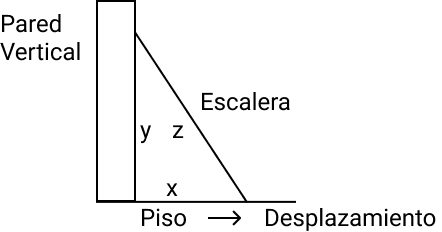
\includegraphics[width=0.5\textwidth]{fmc1.png}}
	\caption{Definición de variables}
	\label{fmc1}
\end{figure}

Donde $z$ es la constante (longitud de la escalera), $x$ la distancia del piso y $y$ la altura de la pared.

Según el diagrama \ref{fmc1}, los datos disponibles son:

\begin{align*}
	 & z=25ft &  & \frac{dx}{dt}=3ft &  & x=1s/ft
\end{align*}

Se relacionan las variables:

\begin{equation*}
	x^2+y^2=z^2
\end{equation*}

Distinguiendo los datos son sobre la horizontal, la incógnita es todo lo que ocurre

\begin{equation*}
	y^2=z^2-x^2\implies y=\sqrt{z^2-x^2}
\end{equation*}


\begin{align*}
	\implies \frac{dy}{dt}=-\frac{x}{y}\cdot \frac{dx}{dt}
\end{align*}

y se sustituyen los datos:

\begin{equation*}
	\frac{dy}{dt}=-\frac{15}{\sqrt{25^2-15^2}}\cdot 3\implies \frac{dy}{dt}=-\frac{45}{\sqrt{400}}=-\frac{45}{20}=-2,25 ft/s
\end{equation*}
